\documentclass[
	a4paper, % Papierformat A4
	12pt, % Schriftgröße 12pt
	twoside, % + BCOR darunter: für doppelseitigen Druck aktivieren, sonst beide deaktivieren
	BCOR=5mm, % Dicke der Bindung berücksichtigen (Copyshop fragen, wie viel das ist)
	fleqn, % flush equations left (--> Formeln linksbündig)
	bibliography=totoc, %bibliographie im Inhaltsverzeichnis
]{report}

\usepackage{pdfpages}
\usepackage{graphicx}
\usepackage{xcolor}
\usepackage[english, main=	ngerman]{babel} % englisch für Zitate auf Englisch
\usepackage[onehalfspacing]{setspace}
\usepackage[utf8]{inputenc}
\usepackage{microtype} % better kerning, word spacing etc
\usepackage{lipsum} % lorem ipsum
\usepackage[round]{natbib}
\usepackage{hyperref}

\bibliographystyle{plainnat}

% \usepackage{fontspec} % custom font (needs compiling via xelatex)
% \setmainfont{Fira Sans}
    
\begin{document}

	%Deckblatt:
	
\includepdf[pages={1}]{Deckblatt/deckblatt.pdf}

	\begin{abstract}
		\lipsum[1]
	\end{abstract}

	%Inhaltsverzeichnis:
	\tableofcontents

	\chapter{Einführung}
	\section{Datenerfassung auf Intensivstationen}

\subsection{Ziel der Arbeit}

Das Ziel der vorliegenden Arbeit ist es, mit Hilfe von maschinellem Lernen ein statistisches Modell zu entwickeln, um anhand von Freitexten medizinische Scores möglichst akkurat vorherzusagen.

\section{Maschinelles Lernen}

Der Begriff Maschinelles Lernen bezeichnet einen modernen Ansatz in der Arbeit an künstlicher Intelligenz. (cite).

hat sich im Zeitalter von Big Data und leistungsstarken Rechnern zu einem der Hauptforschungspunkte der Informatik entwicklt (cite). 

(et al) definiert den Vorgang maschinellen Lernens folgendermaßen:

\begin{quote}
    {\foreignlanguage{english}{A computer program is said to learn from experience E with respect to some class of tasks T and performance measure P, if its performance at tasks in T, as measured by P, improves with experience E.}}
\end{quote}

Im Allgemeinen werden also Algorithmen, die aus großen Datensätzen "lernen" und damit Vorhersagen über unbekannte Daten machen, als maschinelles Lernen bezeichnet.

\subsection{Supervised Learning}

Neben vielen weiteren Methoden stellt Supervised Learning einen zentralen Ansatz im Gebiet des maschinelles Lernen dar.

\subsection{Regression vs Klassifizierung}

Probleme aus dem Bereich des supervised machine learnings lassen sich im Allgemeinen in eine von zwei Kategorien einordnen:

Klassifizierung bezeichnet den Prozess, bei dem ein Datensatz einer oder mehreren Klassen aus einer endlichen Liste möglicher Klassen zugeordnet wird. 

Dieser Ansatz findet beispielsweise bei der automatischen Kategorisierung von E-Mails (Spam oder nicht Spam) oder bei der Erkennung von handschriftlichen Texten (welches Symbol aus einem gegebenen Alphabet ist dargestellt?) Anwendung (CITE). Da es sich bei den betrachteten medizinischen Scores um diskrete, ganzzahlige Werte aus einem endlichen Wertebereich handelt, liegt auch hier die Anwendung eines Klassifizierungs-Verfahrens nahe.

Würde man aber die verschiedenen möglichen Werte eines Scores als separate und voneinander unabhängige Klassen betrachten, so ginge eine wichtige Information über deren Anordnung verloren. Im mathematischen Sinne stellen alle hier betrachteten medizinische Scores Totalordnungen dar. Sie erfüllen also die Anforderungen der Reflexivität, Antisymmetrie, Transitivität und Totalität. Bezeichne $M$ die Menge aller möglichen Werte eines beliebigen medizinischen Scores. Folglich gilt für alle $a,b,c \in M$:

\begin{equation*}
    \begin{aligned}[c]
        a \leq a\\
        a \leq b \land b \leq a \; \Rightarrow \; a=b\\
        a \leq b \land b \leq c \; \Rightarrow \; a \leq c\\
        a \leq b \lor b \leq a
    \end{aligned}
    \qquad
    \begin{aligned}[c]
        \text{(Reflexivität)}\\
        \text{(Antisymmetrie)}\\
        \text{(Transitivität)}\\
        \text{(Totalität)}
    \end{aligned}
\end{equation*}

% \begin{align}
%     a \leq a && \text{(Reflexivität)}\\
%     a \leq b \land b \leq a \; \Rightarrow \; a=b && \text{(Antisymmetrie)}\\
%     a \leq b \land b \leq c \; \Rightarrow \; a \leq c && \text{(Transitivität)}\\
%     a \leq b \lor b \leq a && \text{(Totalität)}
% \end{align}

Damit lassen sich die verschiedenen Scores vergleichen und in ein Verhältnis setzen. So ist ein RASS-Wert\footnote{Richmond Agitation-Sedation Scale} von -4 (Tief sediert) beispielsweise deutlich näher an -3 (mäßig sediert) als an +1 (unruhig). Bei gängigen Verfahren zur Klassifizierung ginge diese Information verloren, da bei Kenngrößen zur Bewertung solcher Modelle nur betrachtet werden kann, ob ein gegebener Eingabetext der richtigen Kategorie (dem richtigen Score) zugeordnet wurde oder nicht. (Da viele der Scores bei der Vergabe zumindest teilweise auch auf dem persönlichen Ermessen des behandelnden Arztes/der behandelnden Ärztin beruht wäre selbst für menschliche Experten eine genaue Zuordnung eines Textes zu einer Punktzahl problematisch.)

Bei dieser Arbeit habe ich mich demnach dafür entschieden, die Vergabe von Scores anhand von Eingabetexten als klassisches Regressionsproblem zu betrachten, und die Ausgaben der Modelle im Zweifelsfall auf den nächstmöglichen ganzzahligen Wert zu runden. Dieser Ansatz fand auch bei früheren Arbeiten, die sich mit ähnlichen Fragestellungen befassten, Anwendung (CITE). Die Abweichung des vorhergesagten Werts eines Modells von dem nächst möglichen Wert stellt somit sogar einen rudimentären Ansatz zur Bewertung der Konfidenz bei der Vergabe einzelner Werte dar.

%siehe: https://stats.stackexchange.com/a/282890 Handelt es sich um \glqq ordinal classification\grqq{}?


% ## 1) Einführung
%   * worum geht es?
%   * Thematik
%     * Problematik der Datenerfassung auf ICUs
%     * bisherige Ansätze, Forschungsarbeiten, Paper etc.
%   * was ist maschinelles lernen?
%     * **Formale Definition von [Mitchell, Tom. (1997). Machine Learning]**
%       * A machine is said to learn from experience E with respect to some class of tasks T and performance measure P...
%     * historischer Kontext (big data, processing power Moore's law etc)
%     * Arten von maschinellem lernen (supervised, unsupervised)
%     * classification vs regression
%     * Bewertung von ML-Modellen
%       * z.b. cross validation
%       * vermeiden: data leakage
%     * (numerische optimierung)
%       * numerische optimierung: Lösungsgraum, Bewertungsfunktion
%       * das Gradientenverfahren
%       * stochastic gradient descend
%     * Herausforderungen von ML für NLP
%     * Machinelles lernen in der medizin
%     * warum ML f. Bearbeitung der Problematik?
	
	
	\chapter{Übersicht über die Daten}
	% \section{Datenerfassung an der Charité}
Auf den Intensivstationen der Charité wird das Patientendatenmanagementsystem COPRA eingesetzt, um Informationen wie etwa Patienten- und Behandlungsdaten zu erfassen, darzustellen und zu verarbeiten. Die Datensätze der vorliegenden Arbeit wurden beim Export aus dem System pseudonymisiert, indem patientenbezogene Daten wie Name und Geburtsdatum entfernt wurden. Insbesondere werden Zeitpunkte nicht in absoluter Form angegebenen, sondern in Relation zum Beginn des Krankenhausaufenthalts des entsprechenden Patienten. Rückschlüsse auf die Identität der Patienten, deren Daten hier betrachtet werden, sind somit ausgeschlossen. Eine Zuordnung der erfassten Werte und Visitentexte untereinander zum selben Patienten bleibt aber durch eine den Patienten eindeutig identifizierenden Zahlenkombination weiterhin möglich.

Nach dem Export lagen die Daten in Form mehrerer Datendateien vor. \texttt{patienten.csv} und \texttt{delir.csv} enthalten Metainformationen über die betrachteten Patienten. Die beiden Dateien \texttt{scores1.csv} und \texttt{scores2.xlsx} geben Aufschluss über die erfassten Scores und eingetragenen Freitexte. Jede Zeile enthält hierbei jeweils die VarID, den betreffenden Patienten, den Zeitpunkt sowie den eigentlichen erfassten Wert. Bei der VarID handelt es sich um einen ganzzahligen Wert, mit der jede Art von auf der Intensivstation erfasstem Wert bzw. eingetragenem Text Charité-intern repräsentiert und eindeutig identifiziert wird \reftbl{table:varids}.

\section{vorliegende Datensätze} \label{section:vorliegende_daten}
Der mir für diese Arbeit zur Verfügung gestellte Datensatz umfasst insgesamt 1357 Patienten-Aufenthalte auf den Intensivstationen der Charité Berlin aus dem Jahr 2017. Jeder Aufenthalt wird über eine numerische, inkrementell aufsteigende Nummer\footnote{in den exportierten Datensätzen als n\_ID bezeichnet} eindeutig identifiziert. Ein Patient, der im Laufe seiner Behandlung mehrere Male auf eine Intensivstation verlegt wird, erhält für jeden separaten Aufenthalt eine neue Identifikationsnummer. Für jeden Patient liegen Informationen über Geschlecht, BMI\footnote{Body-Mass-Index}, Alter zum Zeitpunkt der Aufnahme und ob während des Aufenthalts ein Delir\footnote{F05.* gemäß ICD-10} diagnostiziert wurde vor. Weiterhin ist die Gesamtdauer des Aufenthalts auf der Intensivstation vermerkt, sowie ob der Patient während seines Aufenthalts verstorben ist. Bei den vorliegenden Patienten lag die Mortalität während des Aufenthalts bei etwa 17\% ($n=225$). Die beobachteten Aufenthalte verliefen über Zeiträume von wenigen Stunden bis zu mehreren Monaten. Die mittlere Aufenthaltsdauer während des Beobachtungszeitraums liegt bei etwa 7,2 Tagen, der Median beträgt 3,2 Tage. Fast die Hälfte aller Aufenthalte endete also nach weniger als drei Tagen. Nur etwas mehr als ein Viertel der Patienten ($n=375$) wurden für eine Woche oder länger auf der Intensivstation behandelt.

Für jeden Patienten werden während der Dauer seines Aufenthalts medizinische Scores \refsec{section:scores} bestimmt sowie Visitentexte geschrieben. Die Visitentexte werden digital erfasst und liegen im Unicode-Zeichensatz vor, folgen allerdings im Allgemeinen keinem einheitlichen Muster. Es handelt sich also um unstrukturierte Freitexte, und es liegt im Ermessen der behandelnden Ärzte bzw. Pflegekräfte, einen aussagekräftigen Text zu formulieren. Ebenso können sich Faktoren wie Zeitdruck, Stress oder Ablenkungen durch die Umgebung auf Umfang und Genauigkeit der eingetragenen Texte auswirken \citep{marxIntensivmedizin2015c}.
%Bei den erfassten Scores handelt es sich um medizinische Bewertungssysteme, bei denen die Verfassung des betrachteten Patienten anhand klar definierter Regeln anhand einer Punktzahl bewertet wird(CITE). Häufig beziehen sich die Scores dabei nur auf einen kleinen Teil der Gesamtverfassung des Patienten, beispielsweise auf den Grad der Sedierung (RASS) oder auf das Schmerzempfinden, sofern dieses nicht vom Patienten selber mitgeteilt werden kann (BPS).
%Die in der vorliegenden Arbeit betrachteten Scores weisen es sich um Scores mit einem hohen Grad an Spezifität. Das Ziel solcher Scores ist es nicht, den Gesundheitszustand eines Patienten in seiner Gesamtheit zu erfassen, sondern eher einen klar abgrenzbaren Teilbereich davon \citep{marxIntensivmedizin2015c}. 

Tabelle \ref{table:varids} enthält eine Übersicht über alle Scores und Freitexte, die in dem gegebenen Datensatz erfasst wurden. Es folgt eine detailliertere Beschreibung derjenigen Werte, die für den Inhalt dieser Arbeit besondere Relevanz haben:

\begin{table}[htb] %here > top > bottom
    \centering
    \begin{tabular}{llr}\toprule
        \textbf{VarID}	&\textbf{Name} &\textbf{Wertebereich} \\\midrule
        20512769    & Glasgow Coma Scale (GCS)          & $v \in \interval{3}{15}$ \\
        20512801    & Behavior Pain Scale (BPS)         & $v \in \interval{3}{12}$ \\
        20512802    & Delirium Detection Score (DDS)    & $v \in \interval{3}{35}$ \\
        22085815    & Visite\_ZNS                        & Freitext \\
        22085820    & Visite\_Oberarzt                   & Freitext \\
        22085836    & Visite\_Pflege                     & Freitext \\
        22085897    & Ramsay Sedation Scale             & $v \in \interval{0}{6}$\footnote{Entgegen der ursprünglichen Spezifikation ist an der Charité zusätzlich eine Eintragung des Werts $0$ (für "wach, voll orientiert") möglich.} \\
        22085911    & NRS/VAS (Visual Analogue Scale)   & $v \in \interval{0}{10}$ \\
        22086067    & Vigilanz                          & Freitext* \\
        22086158    & Richmond Agitation Sedation Scale (RASS) & $v \in \interval{-5}{4}$ \\
        22086169    & CAM-ICU                           & $v \in \{	\text{neg.}, \text{pos.}, \text{unmögl.} \}$ \\
        22086170    & BPS-Bewertung                     & Freitext* \\
        22086172    & NRS/VAS Bedingungen               & Freitext* \\\bottomrule
    \end{tabular}

    \caption{Übersicht aller erfassten Scores und Freitexte}
    \label{table:varids}
\end{table}

\paragraph{Glasgow Coma Scale}
Bei der Glasgow Coma Scale (GCS) wird die Schwere einer möglicherweise vorliegenden Bewusstseinsstörung anhand von drei Kategorien (Augenöffnen, verbale Antwort und motorische Reaktion) ermittelt. In jeder Kategorie wird eine Punktzahl ermittelt, die dann zu einem Endergebnis aufsummiert werden. Insgesamt sind so Werte zwischen einschließlich 3 und 15 möglich \citep{teasdaleAssessmentComaImpaired1974,marxIntensivmedizin2015c}.

\paragraph{RASS}
Die Richmond Agitation Sedation Scale (RASS) ist eine zehnstufige Messzahl, die den Grad der Sedierung eines Intensivpatienten beschreibt. Mögliche Werte liegen zwischen $-5$ ("unarousable"/"nicht erweckbar") und $4$ ("combative"/"streitlustig"). Bei den betrachteten Patienten wurde der Wert $0$ ("aufmerksam und ruhig") am häufigsten erfasst, was dem erwünschten Wert entspricht, solange keine Sedierung indiziert ist. Die Autoren der Skala empfehlen eine Reihe von Stimuli, die dem Patienten präsentiert werden sollen, um eine besonders genaue Bestimmung des richtigen Wertes zu ermöglichen \citep{sesslerRichmondAgitationSedation2002a}. Die RASS weist eine hohe Reliabilität und Validität auf und gilt im deutschsprachigen Raum als Goldstandard zum Monitoring der Sedierungstiefe \citep{marxIntensivmedizin2015c, muellerAnalgesieSedierungUnd2015}.

% \paragraph{CAM-ICU}
% bla bla bla %https://www.ai-online.info/images/ai-ausgabe/2009/10-2009/2009_10_592-600_Confusion%20Assessment%20Method%20for%20Intensive%20Care%20Unit%20zur%20routine-maessigen%20Kontrolle%20.pdf
% Eine Besonderheit des CAM-ICU unter den vorliegenden Daten ist, dass es sich hierbei um einen binären Wert handelt:)

% \paragraph{NRS/VAS (Visual Analogue Scale)}
% bla bla bla

\paragraph{Visite\_ZNS, Visite\_Oberarzt und Visite\_Pflege}
bla bla bla (Fridtjof fragen)

\begin{figure}[htb]
    \captionsetup[subfigure]{labelformat=empty, justification=centering}

    \centering
    \subfloat[Behavior Pain Scale]{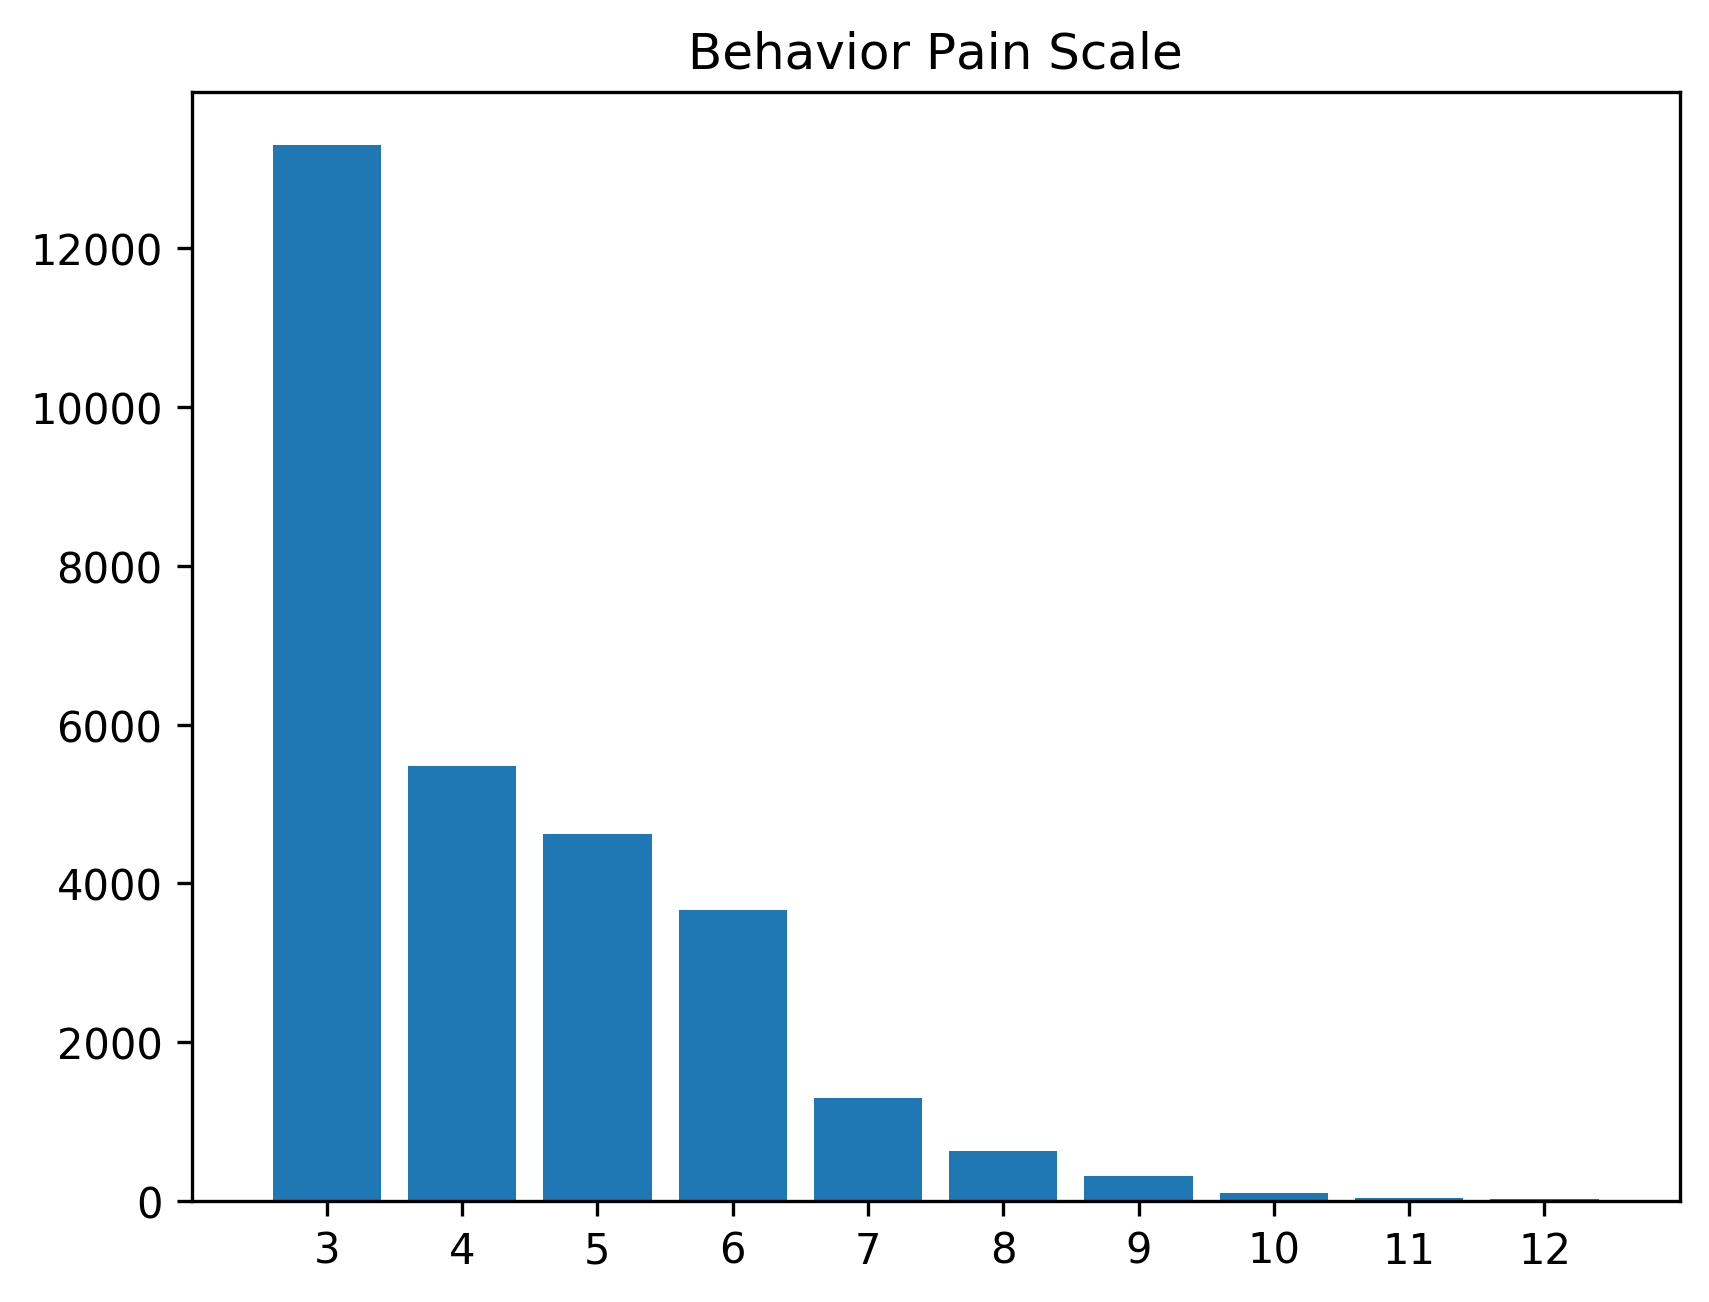
\includegraphics[width=0.35\textwidth]{score_histograms/hist_Behavior_Pain_Scale}} \qquad
    \subfloat[CAM-ICU]{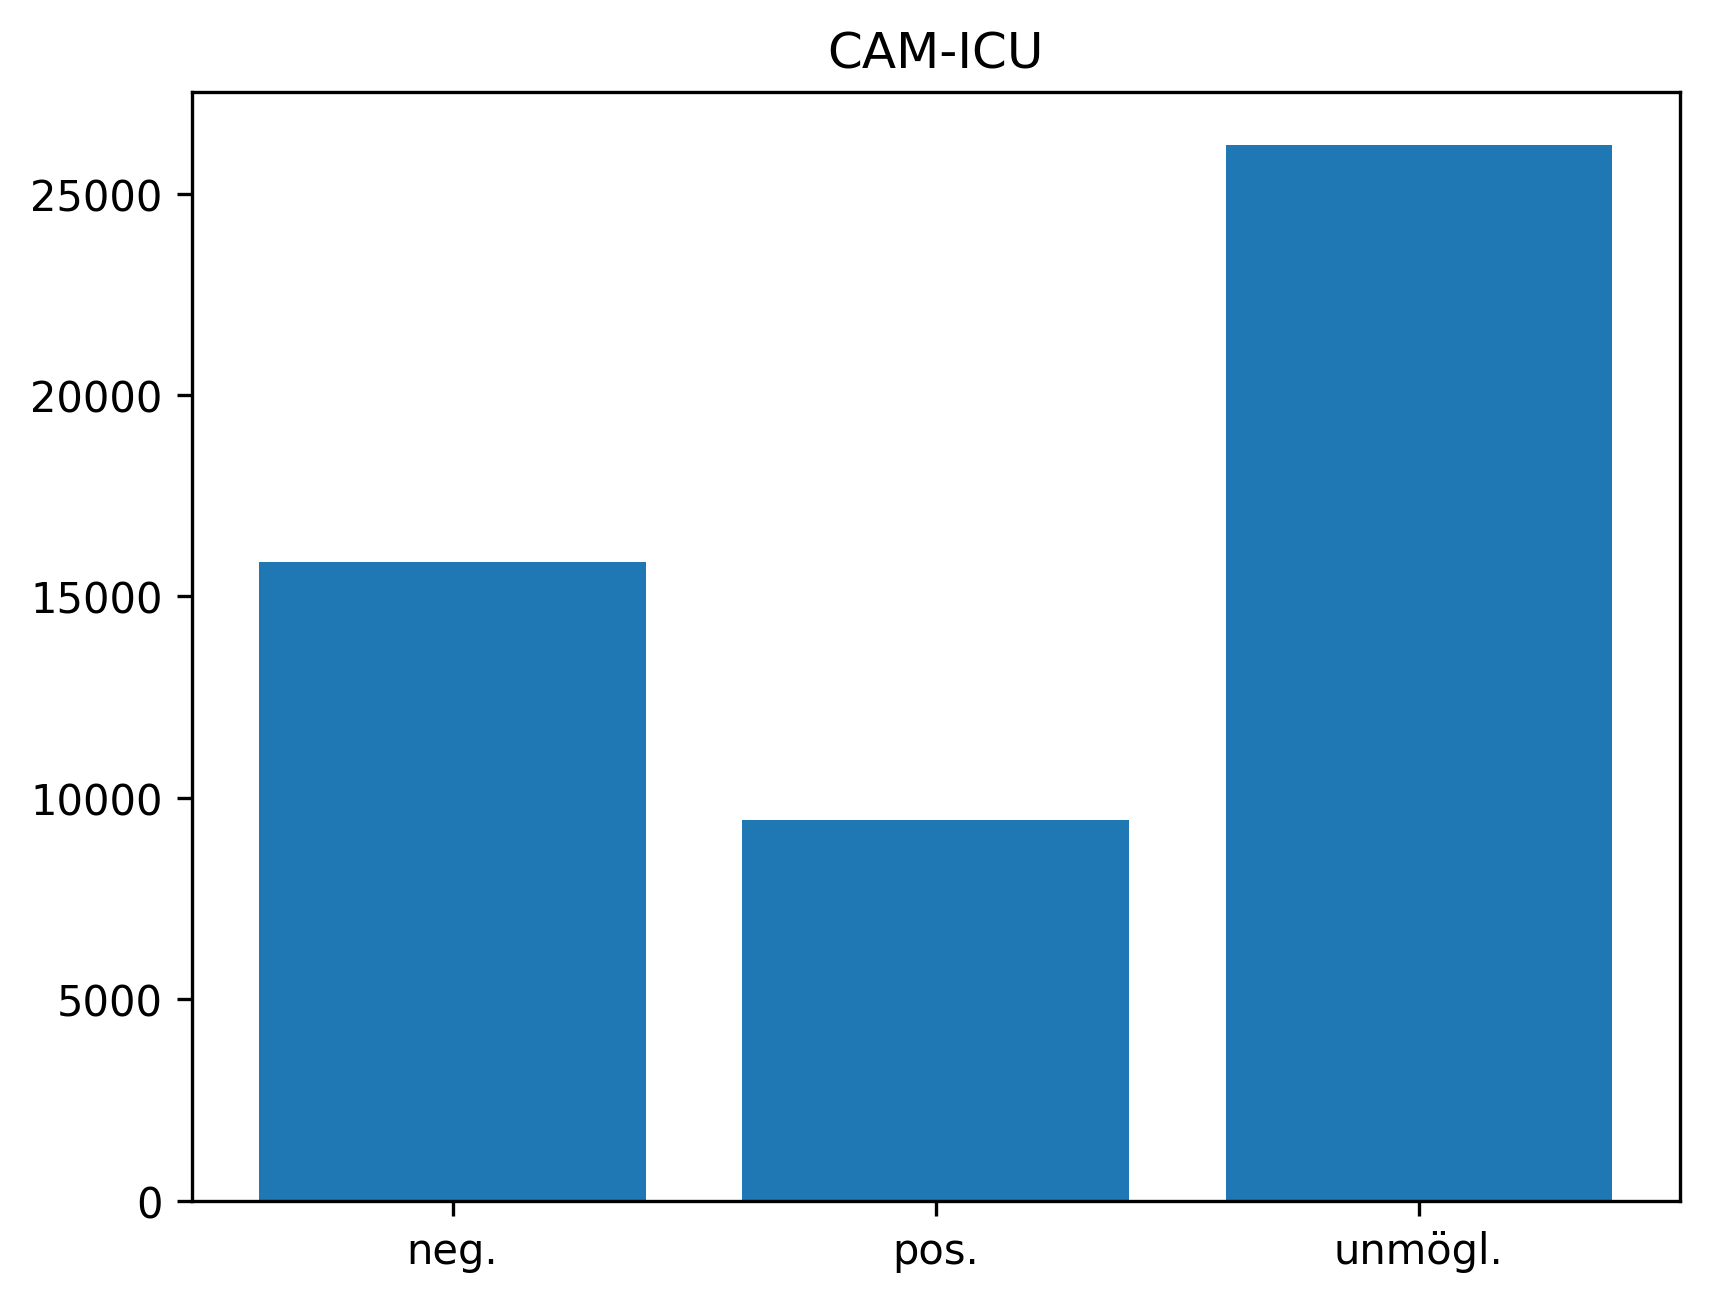
\includegraphics[width=0.35\textwidth]{score_histograms/hist_CAM-ICU}} \\ % linebreak here
    % \subfloat[Delirium Detection Score]{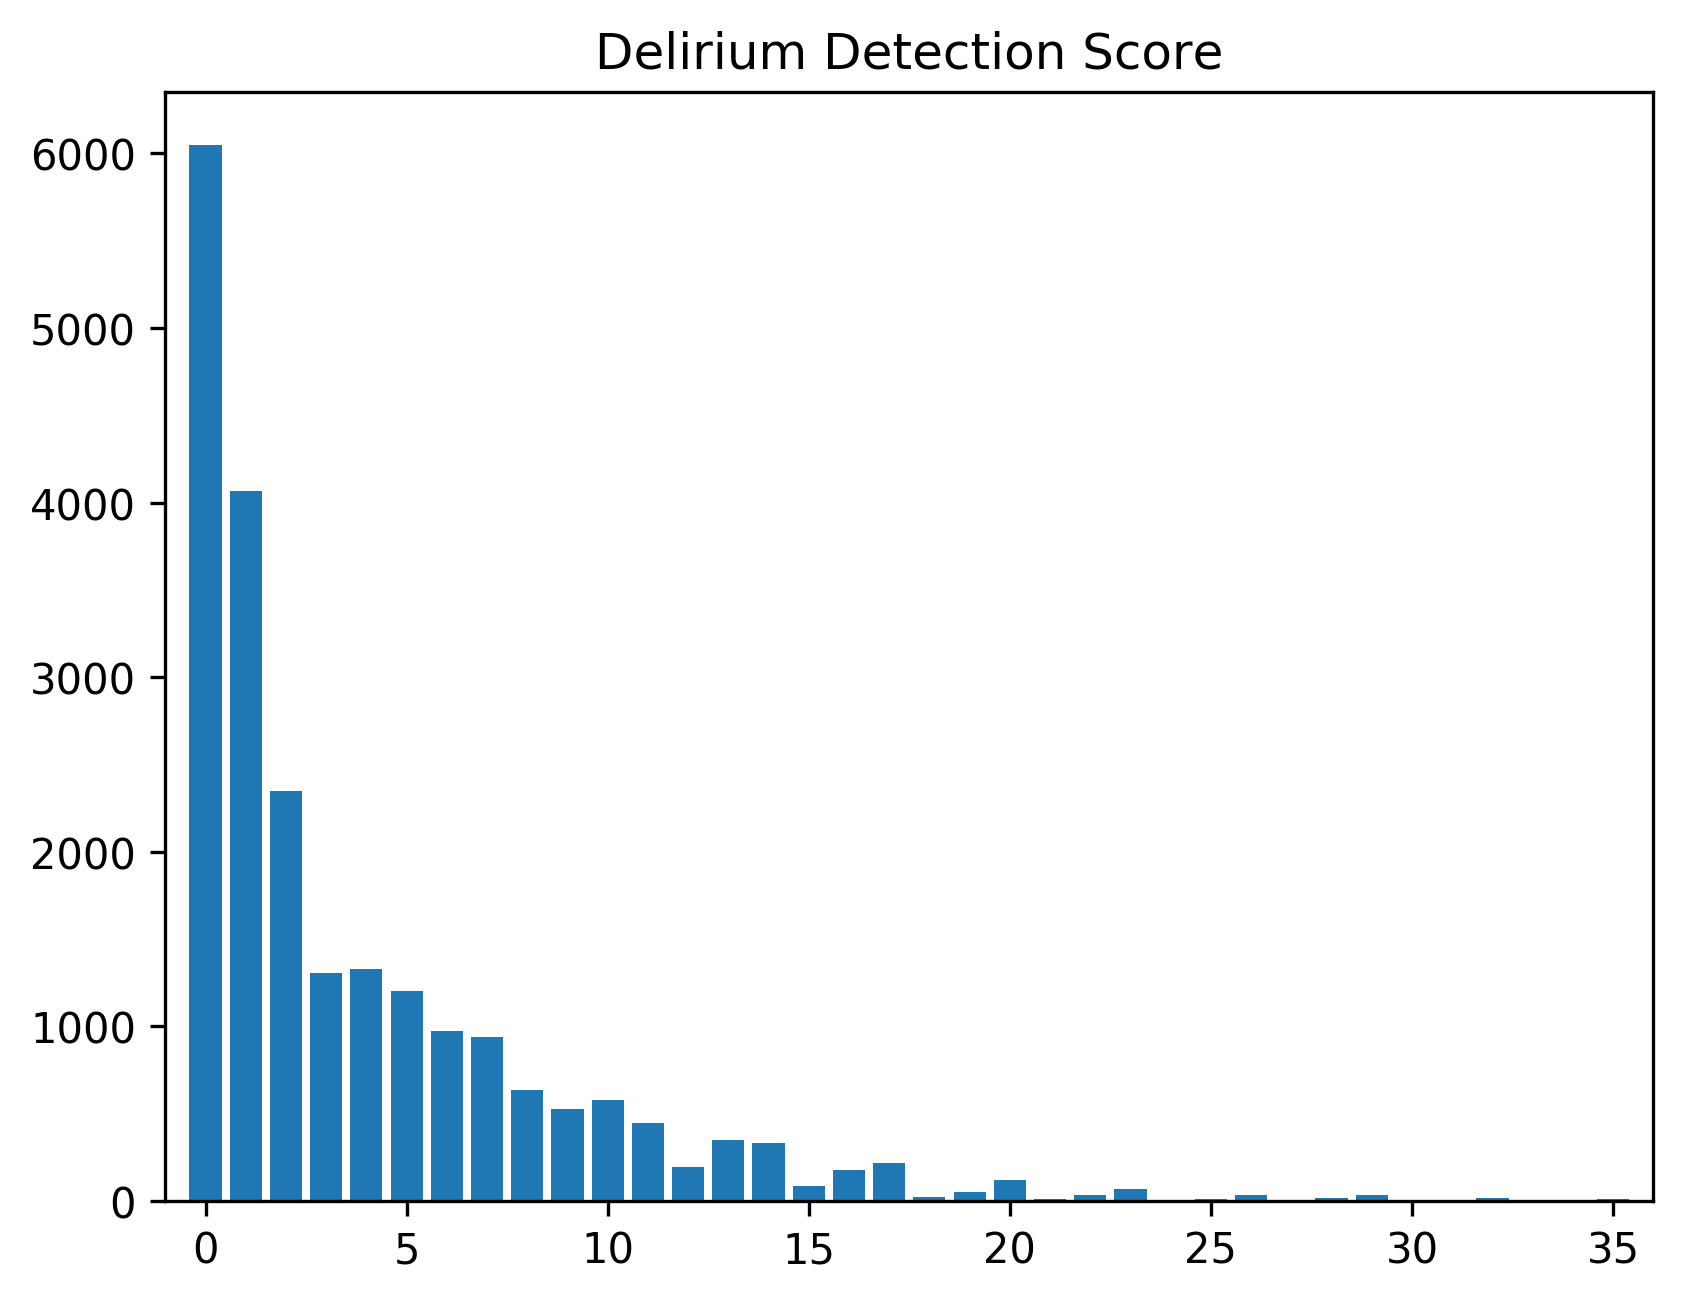
\includegraphics[width=4.75cm]{score_histograms/hist_Delirium_Detection_Score}} \\ % linebreak here
    \subfloat[Glasgow Coma Scale]{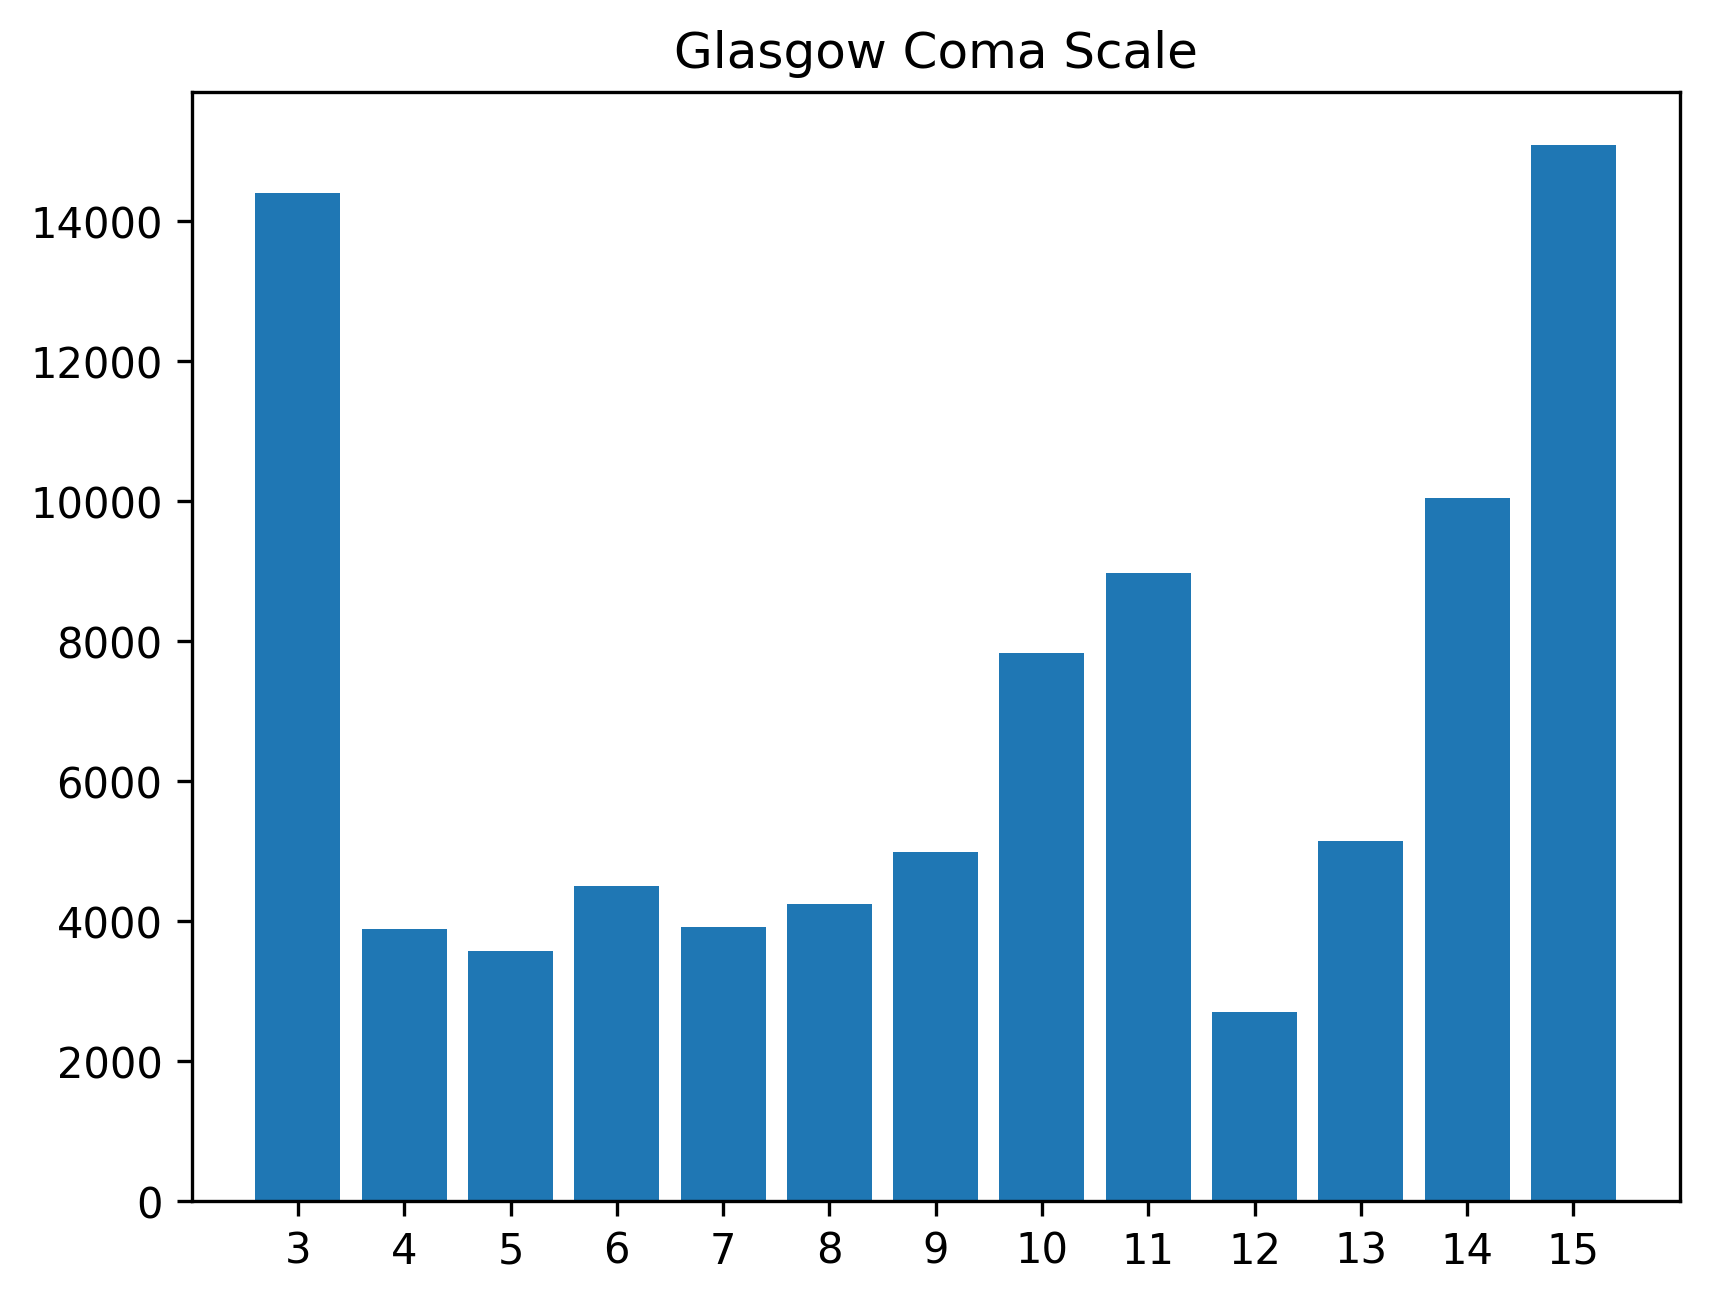
\includegraphics[width=0.35\textwidth]{score_histograms/hist_Glasgow_Coma_Scale}} \qquad
    \subfloat[Richmond Agitation Sedation Scale]{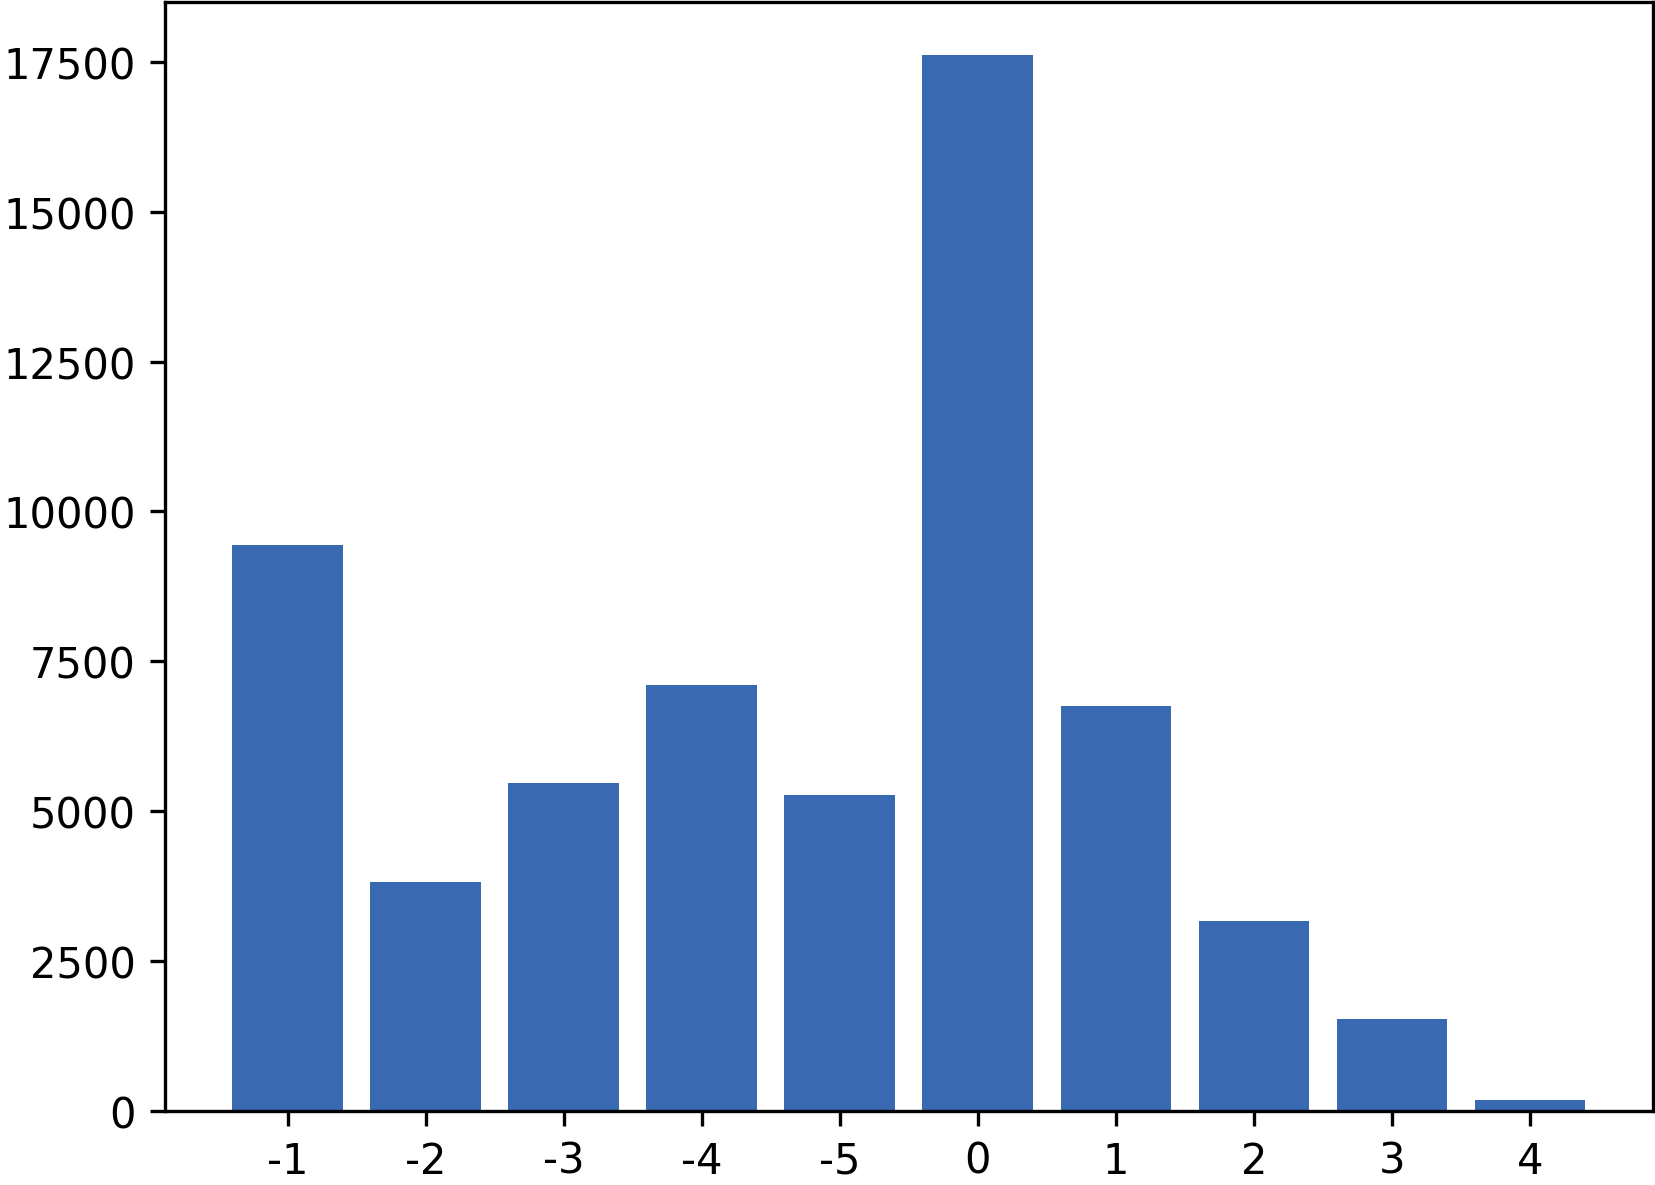
\includegraphics[width=0.35\textwidth]{score_histograms/hist_Richmond_Agitation_Sedation_Scale}}
    % \subfloat[Visual Analogue Scale]{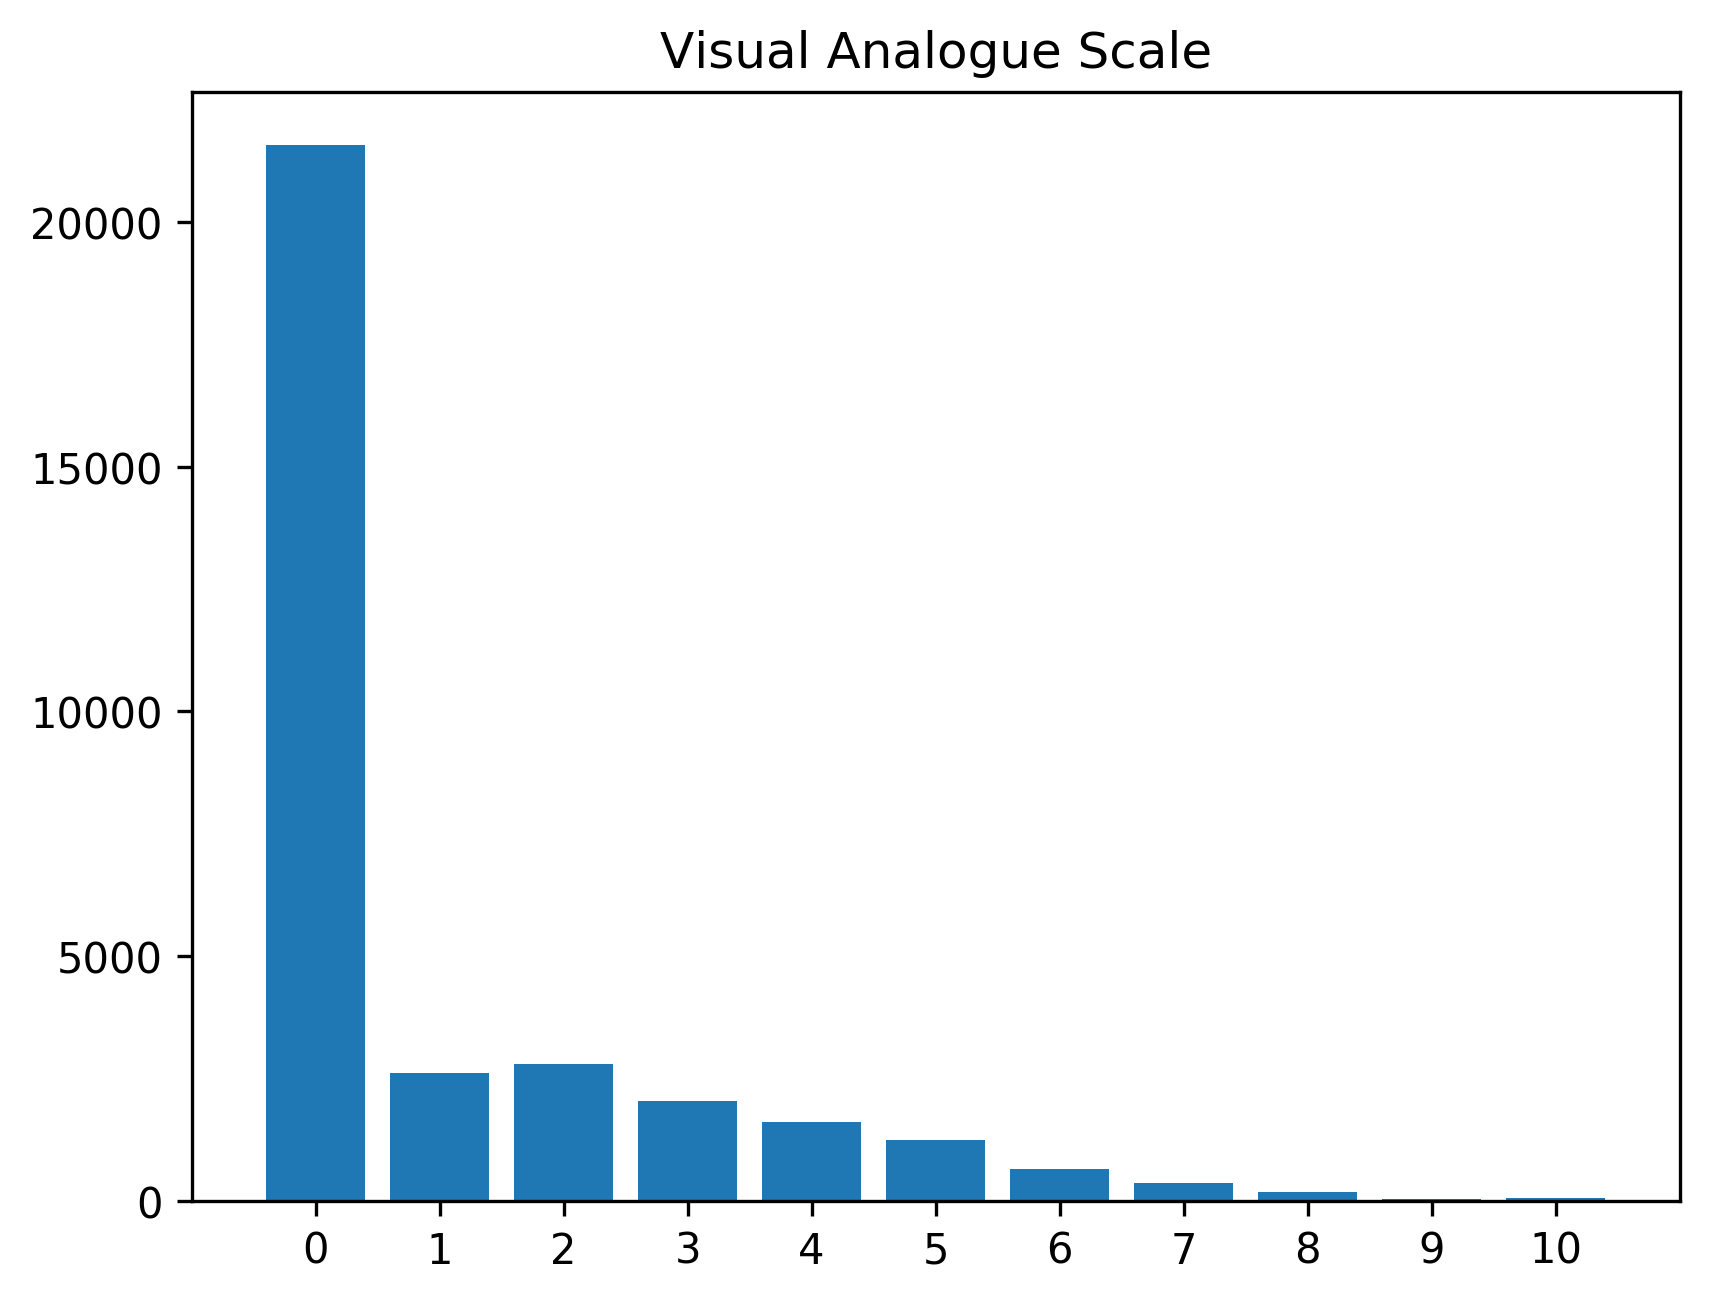
\includegraphics[width=4.75cm]{score_histograms/hist_Visual_Analogue_Scale}} \\
    \caption{Histogramme einiger erfassten Scores}
    \label{fig:score_histograms}
\end{figure}

% \subsection{Exemplarische Vorstellung eines Patienten} %z.b. 0430
% Aufenthalt des Patienten hier detailliert beschreiben, und seinen Scatterplot einfügen (aber noch ohne Pfeile).

\section{Generierung von Schlüssel-Wert-Paaren}
Eine besondere Herausforderung stellte dar, dass die verschiedenen Scores und Texte zu unterschiedlichen Zeiten und unabhängig voneinander eingetragen werden (siehe Abbildung \ref{fig:pat40_scatter}).
%Die Informationen über Zeitpunkt, Art der Eintragung (VarID) sowie der eigentliche Wert liegen jeweils in Form von Tripeln in den entsprechenden Log-Dateien vor. Bei den Visitentexten enthalten die Tripel den entsprechenden Text als Wert der Eintragung.
Um ein Machine-Learning Modell mit einer hohen Dimensionalität der Eingabevektoren zu trainieren ist eine hohe Anzahl von Trainingspaaren notwendig. Im konkreten Fall dieser Arbeit enthält jedes Wertepaar einen Visitentext sowie einen medizinischen Score, der den in dem Text angegebenen Informationen über die Verfasssung des Patienten möglichst genau entspricht. Zusammen bilden diese Paare die Grundlage der Modelle, selbstständig noch nicht gesehene Texte bewerten zu können. Aufgrund der zeitlichen Unterschiede zwischen den Eintragungen von Texten und Scores erwies sich allerdings ebenjene Zuordnung zueinander als nicht trivial. 

\begin{figure}[htb]
    \captionsetup{justification=centering}
    \centering
    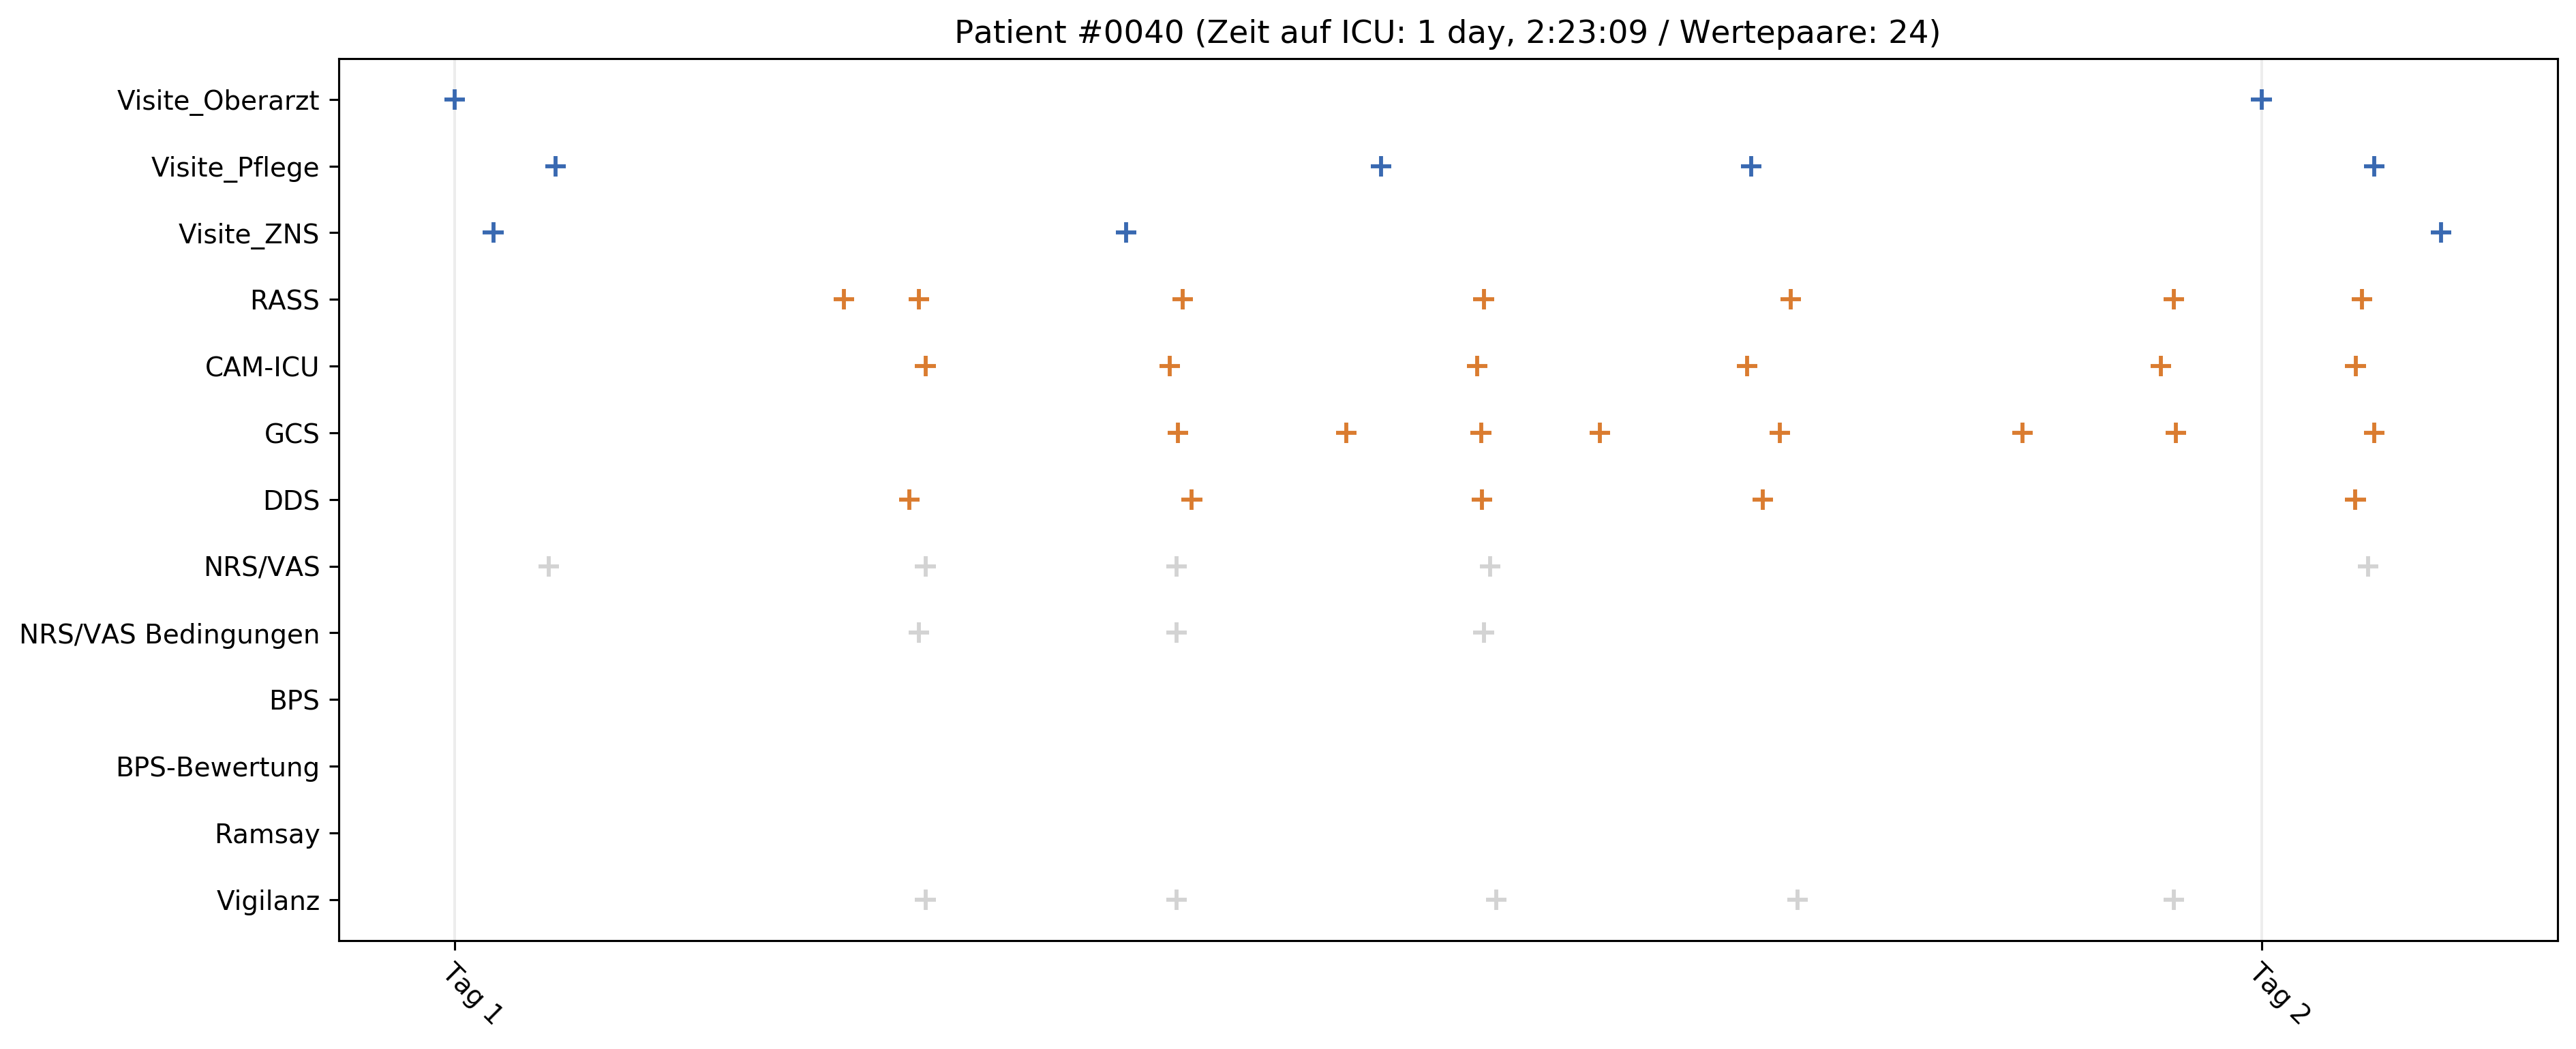
\includegraphics[width=\textwidth]{patienten_scatters/patient_0040_noarrows.png}
    \caption{Die Visitentexte (blau) und Scores (orange) werden zeitlich unabhängig voneinander eingetragen bzw. erfasst.}
    \label{fig:pat40_scatter}
\end{figure}

Ein möglicher naiver Ansatz wäre es, für einen bestimmten Zeitraum den Mittelwert aller Erhebungen eines Scores zu ermitteln, sowie alle Visitentexte, die in diesem Zeitraum erfasst wurden, aneinanderzuhängen. Wählt man beispielsweise einen Zeitraum von 4 Stunden, erhielte man so für jeden Patient, Visitentext und Score 6 Wertepaare pro Tag, mit denen sich ein statistisches Modell trainieren ließe.

Aus zwei Gründen habe ich mich allerdings für einen anderen Ansatz entschieden: Zum einen ist es durchaus möglich, dass sich ein bestimmter Wert innerhalb von wenigen Sekunden stark verändert -- beispielsweise die RASS, wenn die Sedierung eines Patienten eingeleitet wird. Derartige Informationen könnten verloren gehen, wenn man von vornherein nur feste Zeiträume betrachtet. Weiterhin gibt es zwischen individuellen Patienten hohe Schwankungen in der Frequenz und Häufigkeit, in denen bestimmte Scores erfasst werden (siehe Abbildung \ref{fig:pat_example_scatterplots}). Würde man einen festen Zeitraum bestimmen, in welchem die Werte stets zusammengefasst werden, so würden unter Umständen viele Informationen verloren gehen. Auf der anderen Seite kann es vorkommen, dass ein Score in einem Zeitraum gar nicht oder sehr selten erfasst wurde. Die Gefahr, dass sich die Erhebung eines Score dann auf einen ganz anderen Zeitpunkt als ein im gleichen Zeitraum geschriebener Text bezieht, wäre damit sehr groß. Die Korrelation zwischen Inhalt des Visitentexts und des Scores wäre womöglich sehr gering, und die entstehenden Wertepaare dementsprechend ungeeignet, ein effektives Modell zu trainieren.

Zur Generierung der Wertepaare habe ich mich demnach für eine andere Methodik entschieden. Die Implementierung liegt hierfür in \texttt{skripte/find\_training\_pairs.py} vor. Jeder Erhebung eines Scores wird derjenige Visitentext zugeordnet, der zeitlich betrachtet am nächsten zu dem erhobenen Score eingetragen wurde. Dabei kann der Text sowohl vor als auch nach der Eintragung des Scores verfasst worden sein. Weiterhin werden \texttt{Visite\_Pflege}, \texttt{Visite\_ZNS} und \texttt{Visite\_Oberarzt} unabhängig voneinander betrachtet, sodass pro Eintragung eines Scores jeweils eine Zuordnung zu jedem der drei Texte erfolgt. In Abbildung \ref{fig:pat_example_scatterplots} sind diese Zuordnungen durch Pfeile dargestellt. Beim späteren Training der Modelle werden dann nur solche Trainingspaare betrachtet, die den gewünschten Eingabetext beinhalten. Außerdem kann es auch mit dieser Methode vorkommen, dass in einigen Ausnahmefällen die Eintragungen von Score bzw. Text mit einem großen zeitlichen Abstand erfolgt sind. Deswegen wird für jedes Wertepaar zusätzlich die zeitliche Differenz der beiden Eintragungen gespeichert. Das ermöglicht, dass vor dem Trainining eines Modells nur solche Wertepaare selektiert werden, deren zeitlicher Abstand unter einem festgelegten Maximalwert liegt. Da zunächst alle erdenklichen Wertepaare vorliegen kann dieser maximale Abstand je nach Bedarf besonders groß oder klein gewählt werden, beispielsweise dann, wenn ein Modell eine besonders hohe Anzahl an Trainingspaaren benötigt. Abbildung \ref{fig:n_pairs_by_max_offset} zeigt die Anzahl der Wertepaare pro Kategorie von Eingabetext je nach maximal erlaubter Zeit zwischen den beiden Eintragungen.

\begin{figure}[htp]
    \captionsetup{justification=centering}
    \centering
    \subfloat{{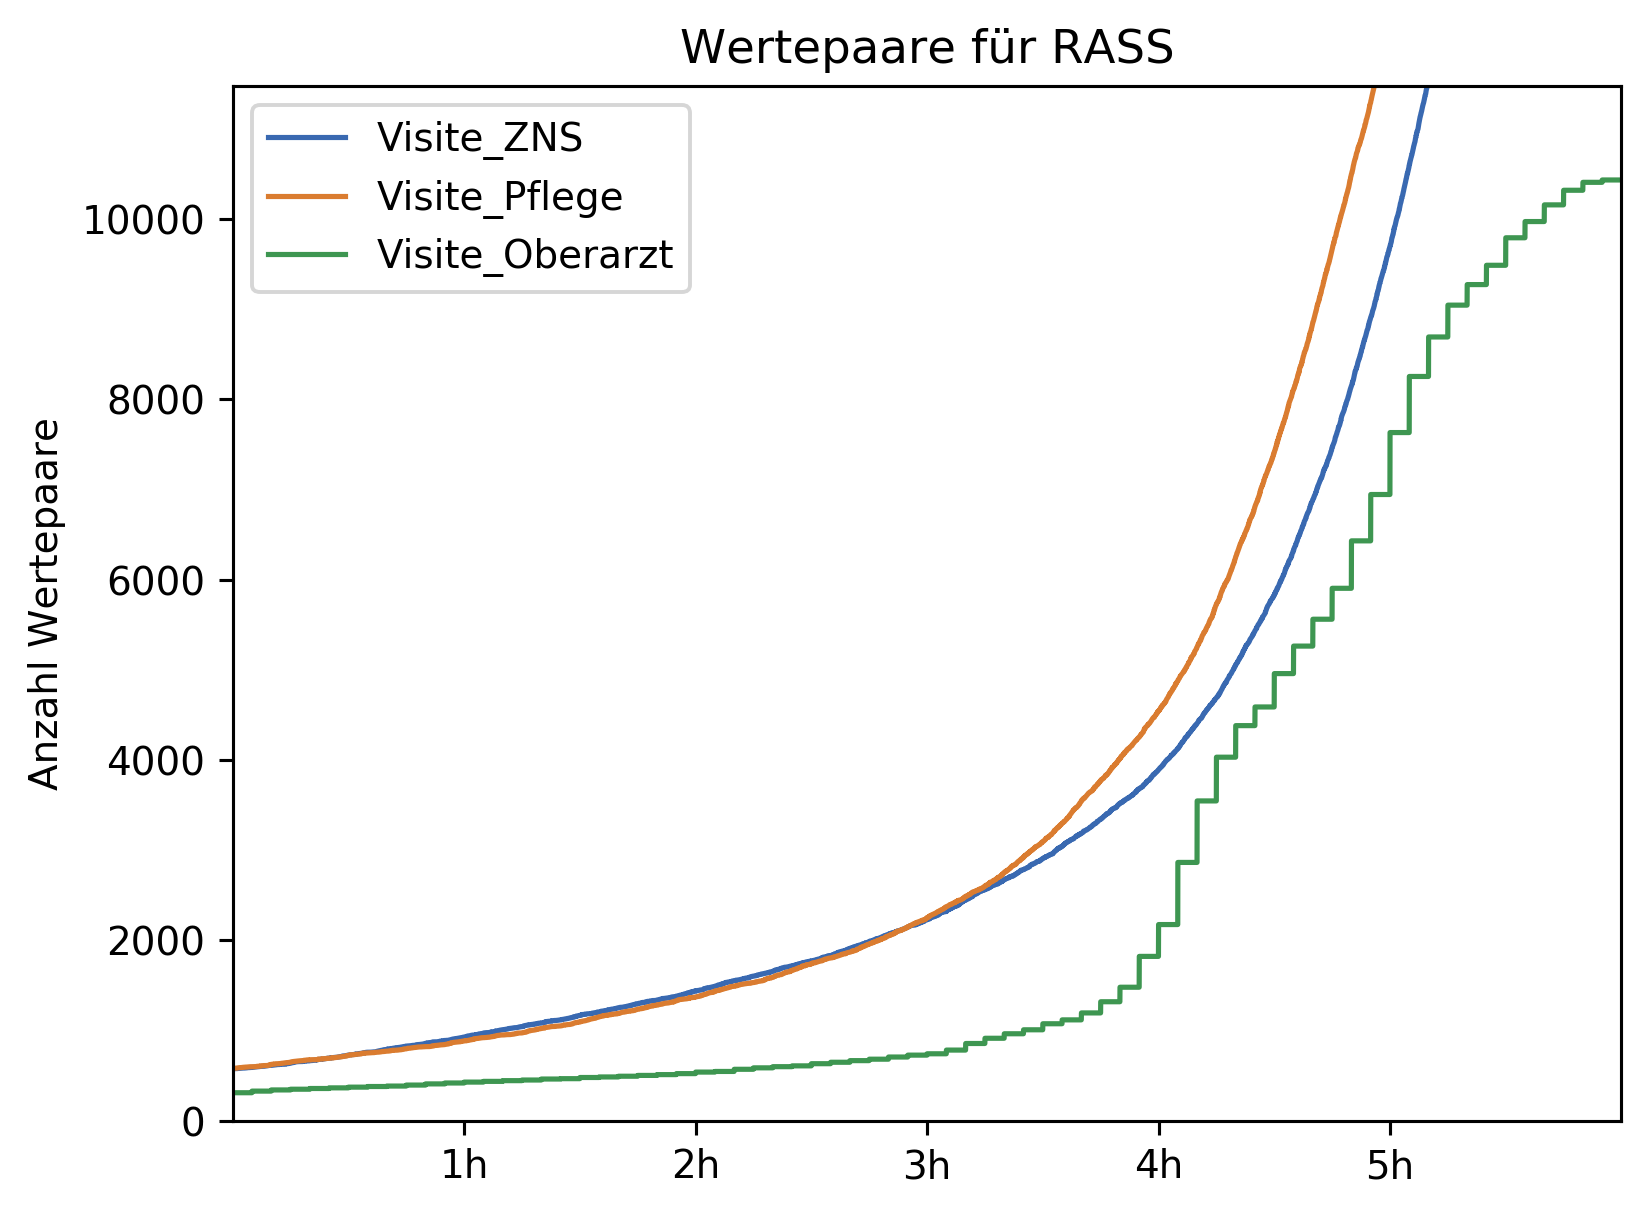
\includegraphics[width=7cm]{pairs_by_max_minRASS.png} }}
    \quad
    \subfloat{{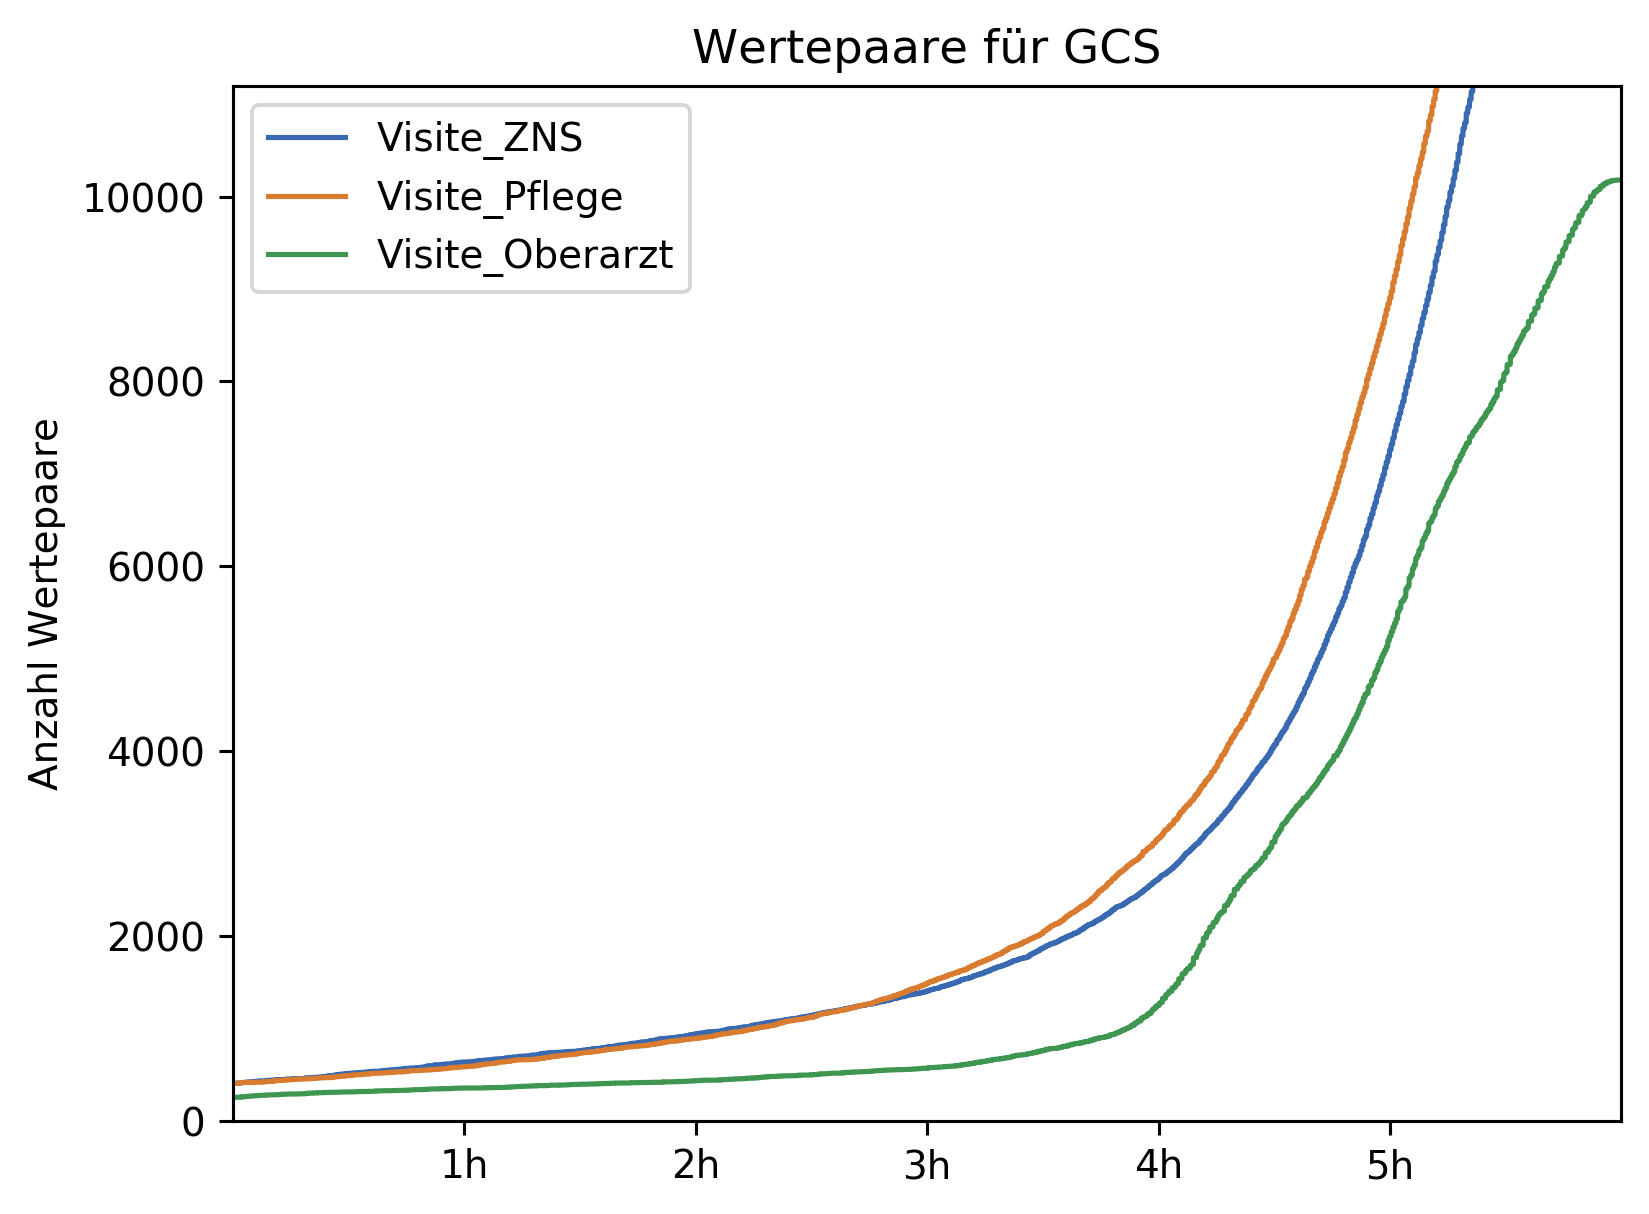
\includegraphics[width=7cm]{pairs_by_max_minGCS.png} }}
    \caption{Anzahl Wertepaare bei maximal zulässiger Differenz zwischen \mbox{Zeitpunkten}}
    \label{fig:n_pairs_by_max_offset}
\end{figure}
% Möglichkeit das noch zu verbessern: statt alle texte innerhalb von z.b. 6h eines Textes zu betrachten: solche ausschließen, die näher an einer anderen erfassung des gleichen scores liegen? 

% Hier Bild mit 4 Patienten-Scatterplots! Bildbeschreibung: "Patient X ist der Patient, dessen Aufenthalt in Sektion 2.2.2 detailliert vorgestellt wurde."
\begin{figure}[p]
    \centering
    \subfloat{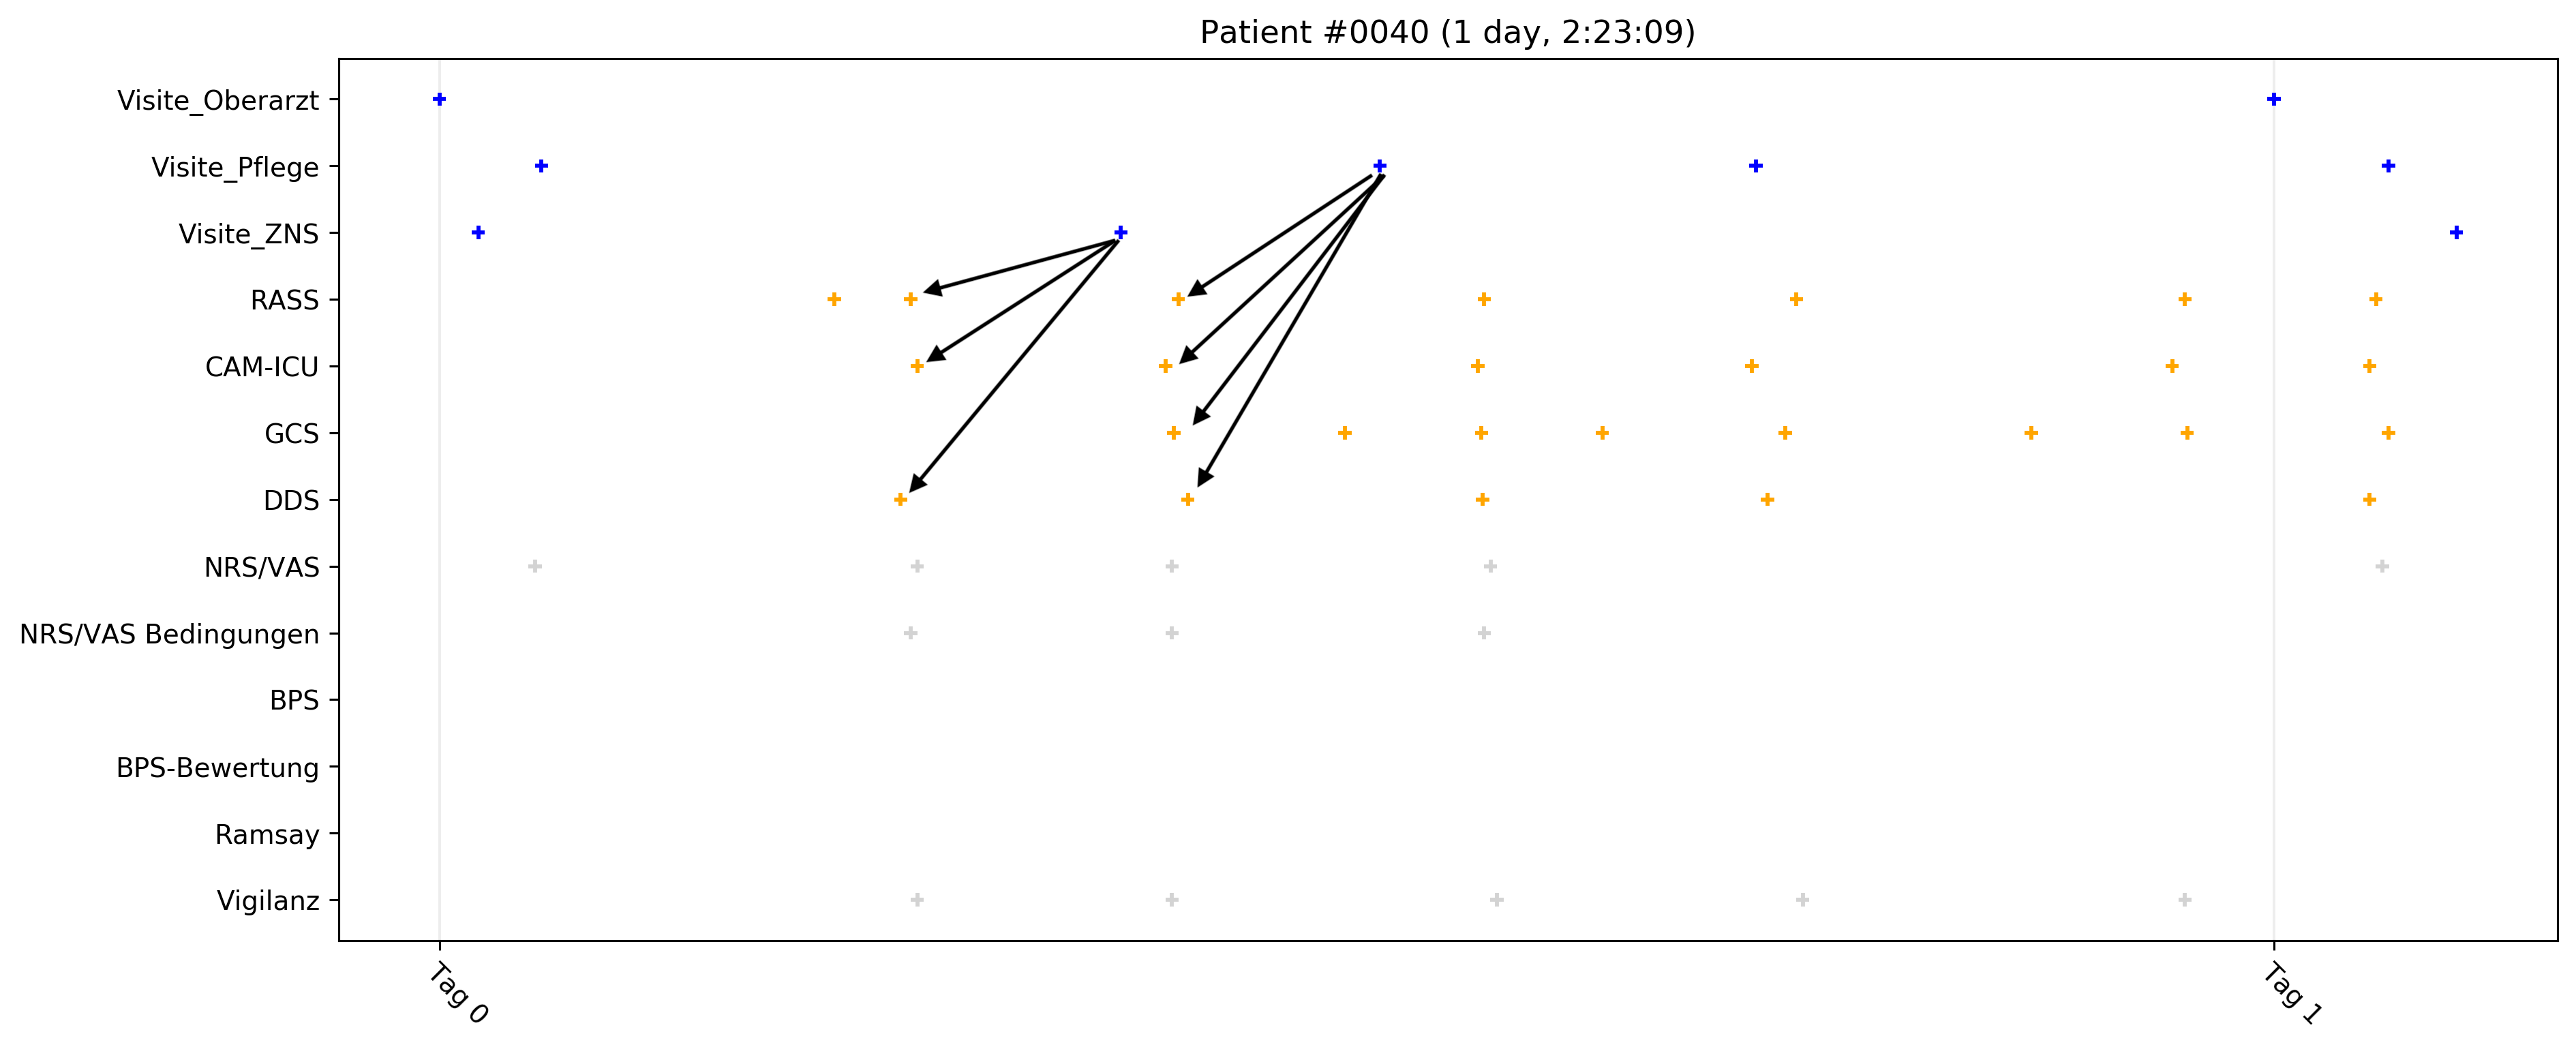
\includegraphics[height=1.87in]{patienten_scatters/patient_0040}} \\
    \subfloat{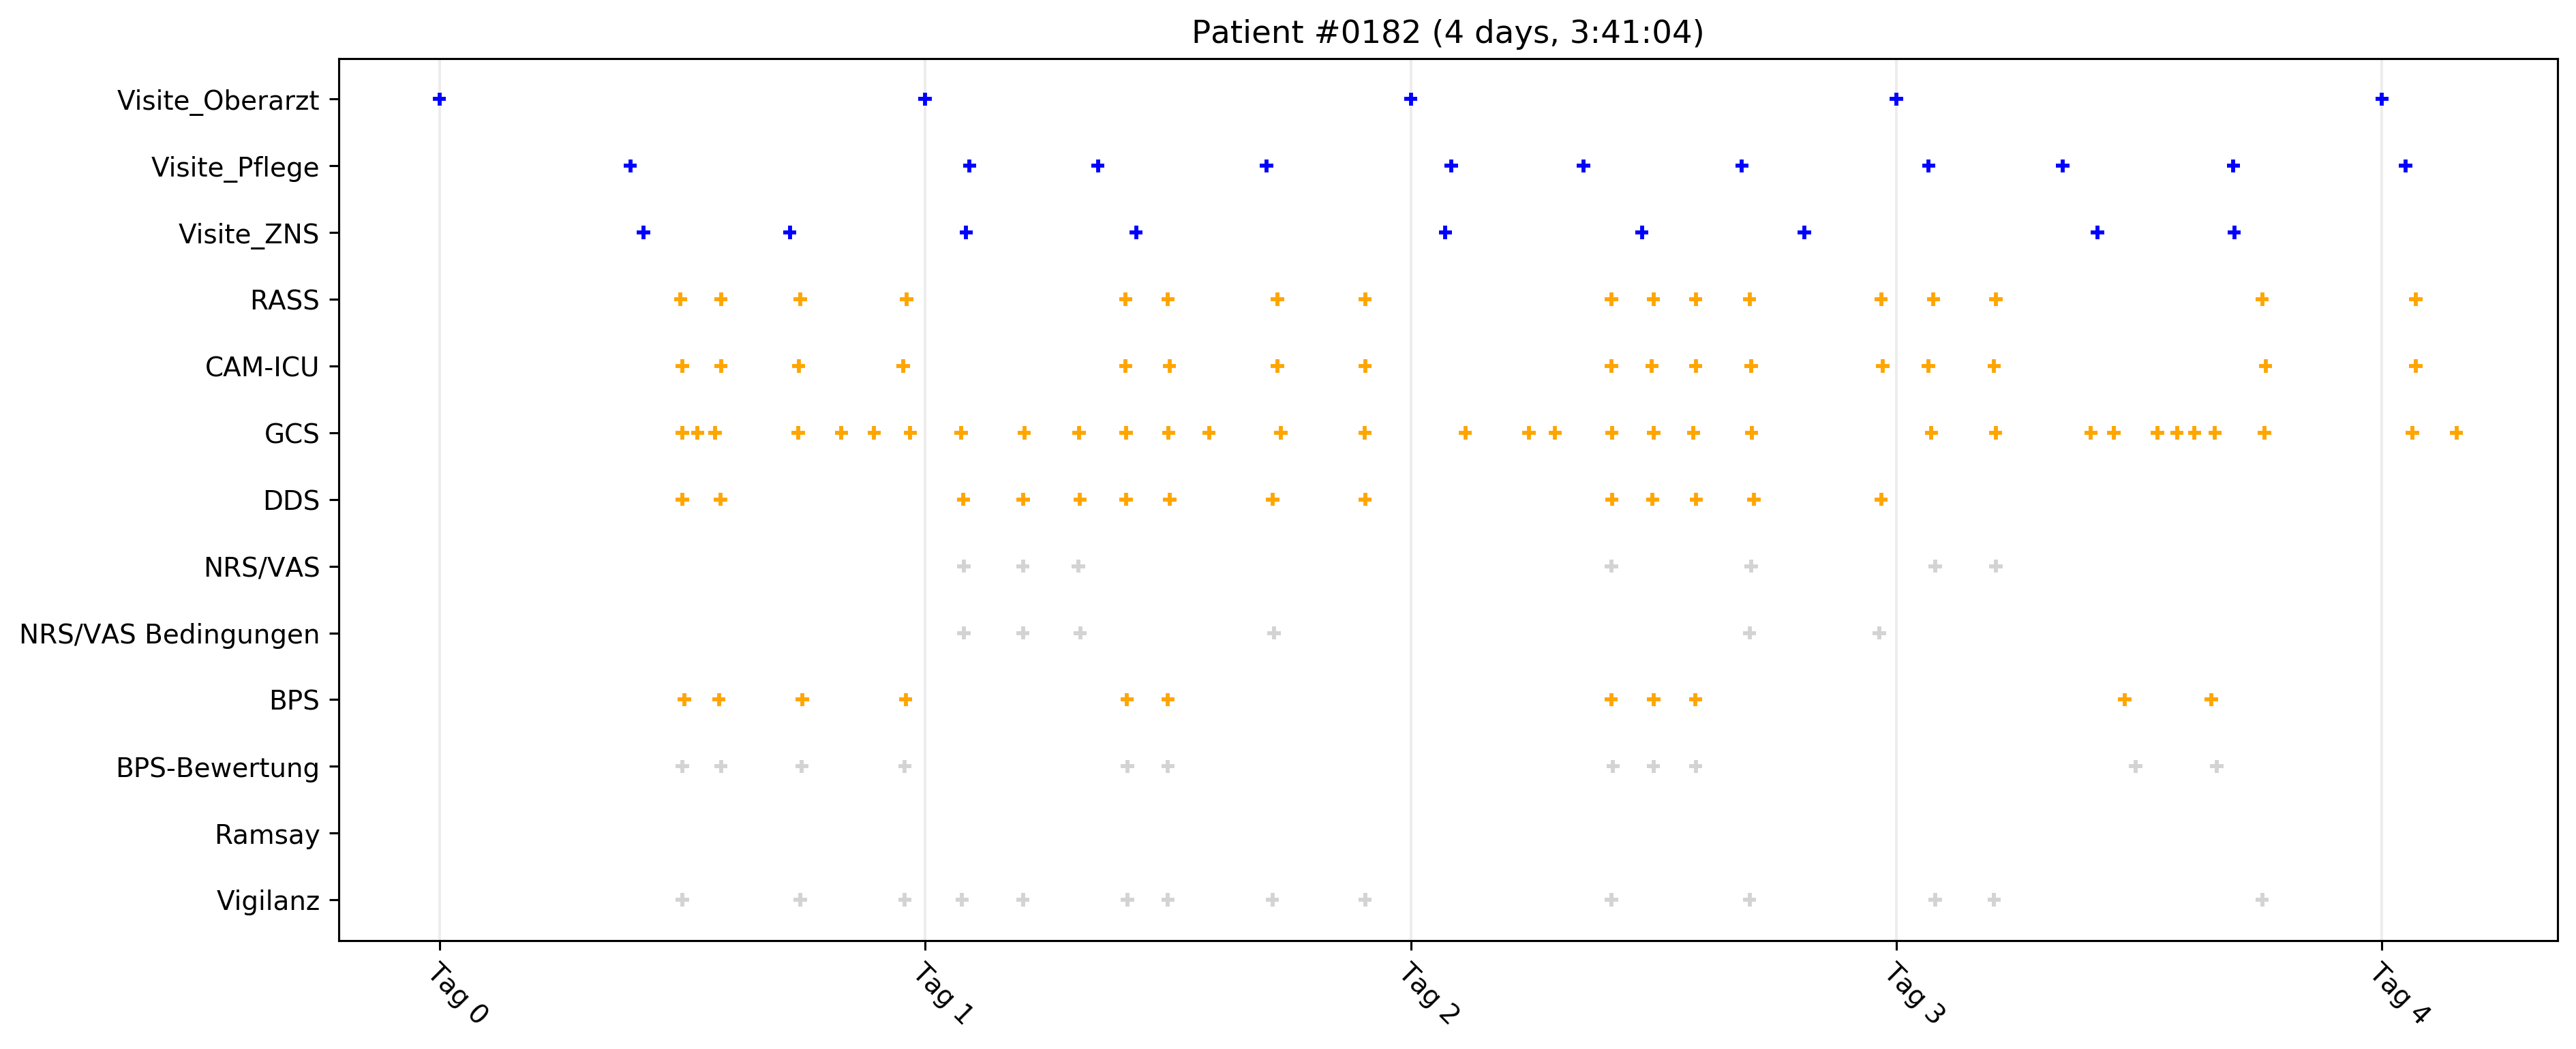
\includegraphics[height=1.87in]{patienten_scatters/patient_0182}} \\
    \subfloat{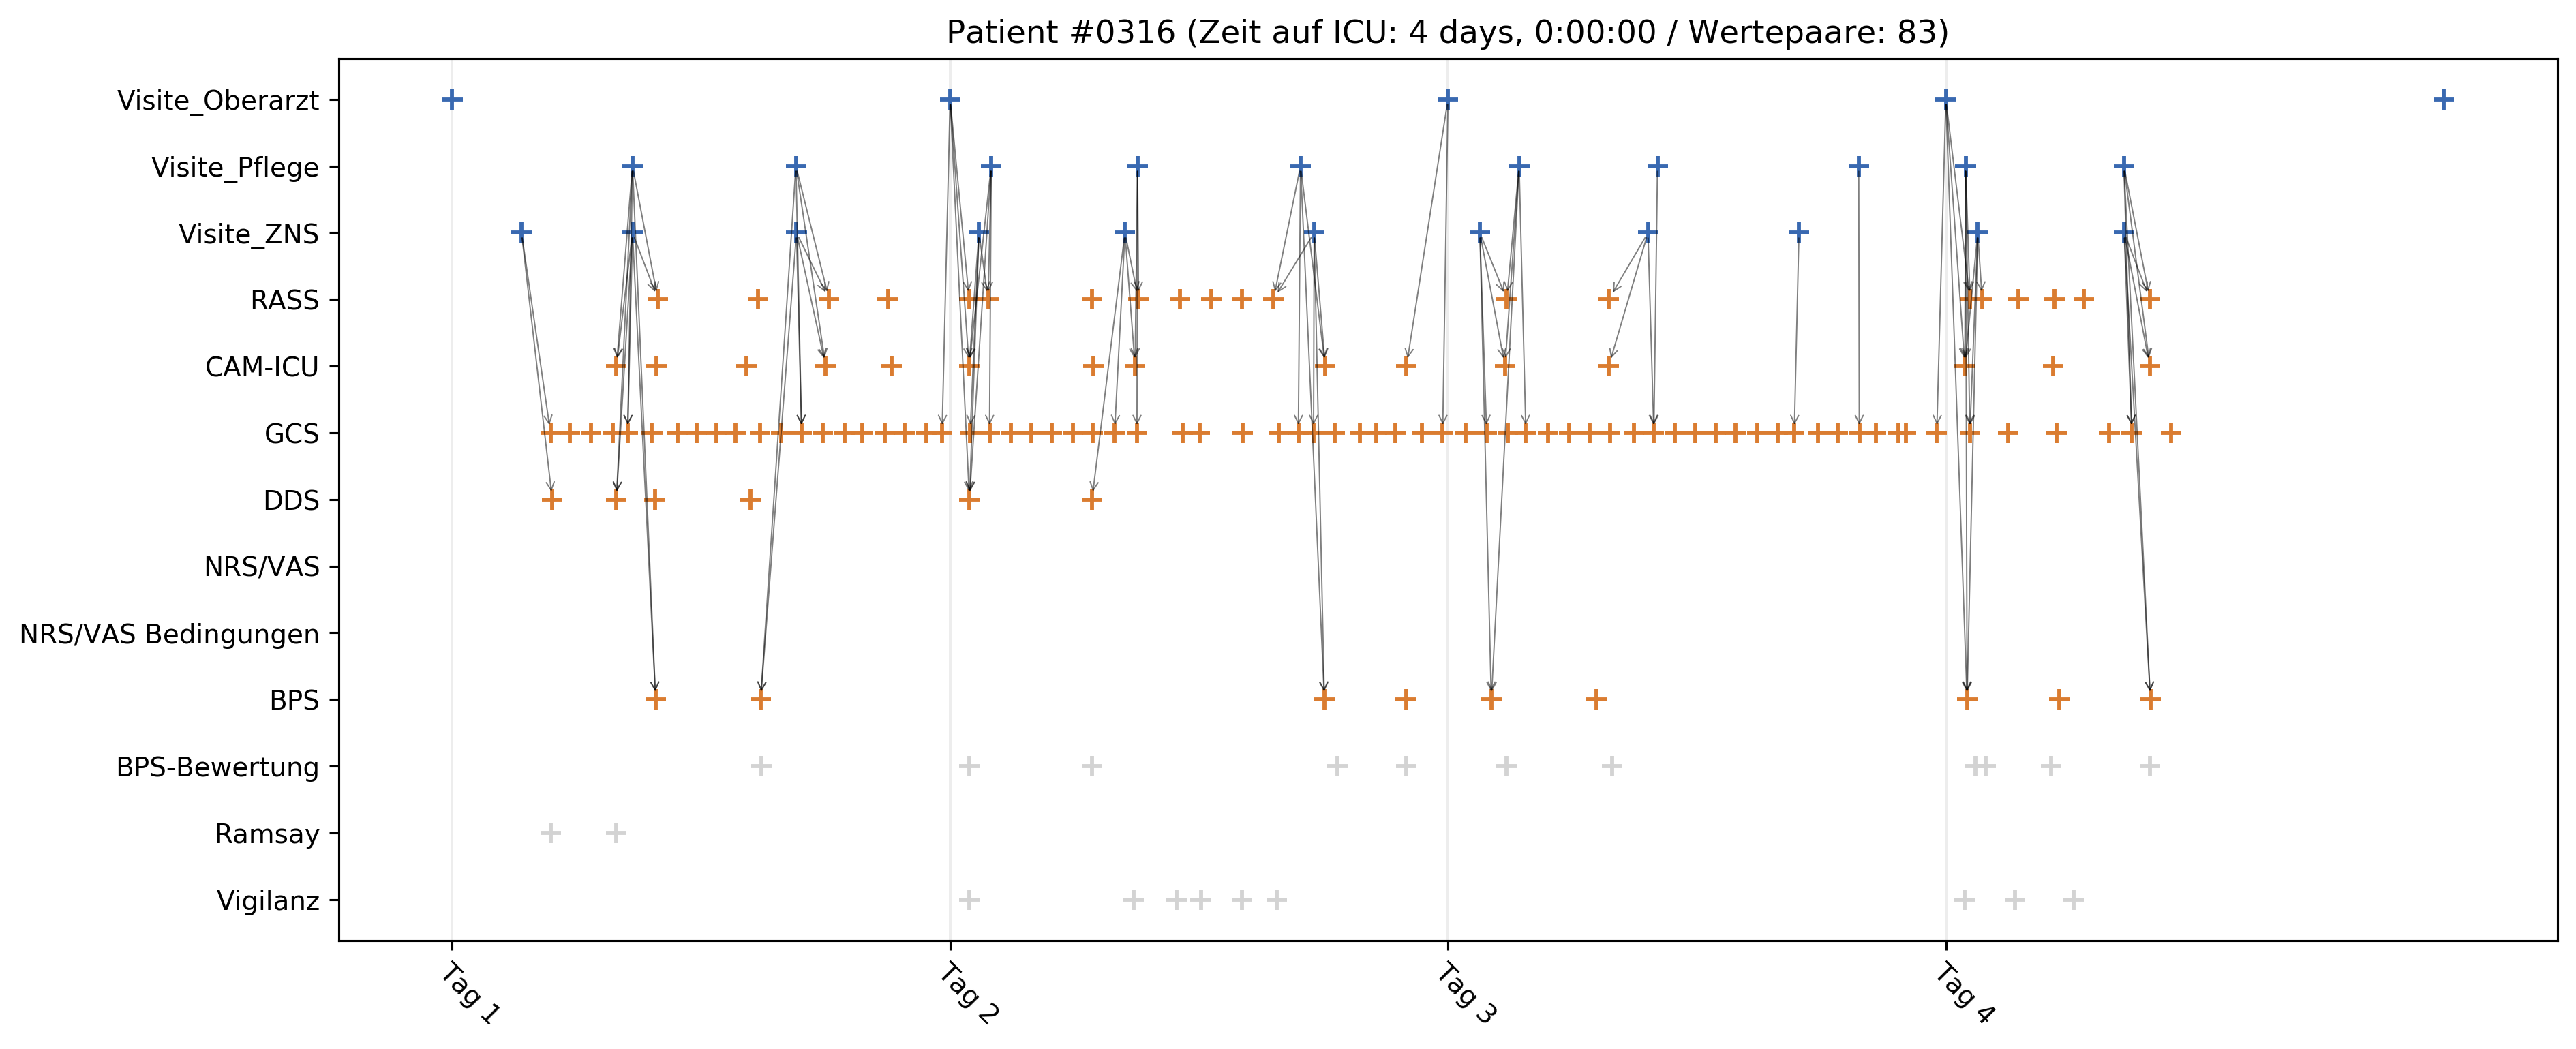
\includegraphics[height=1.87in]{patienten_scatters/patient_0316}} \\
    \subfloat{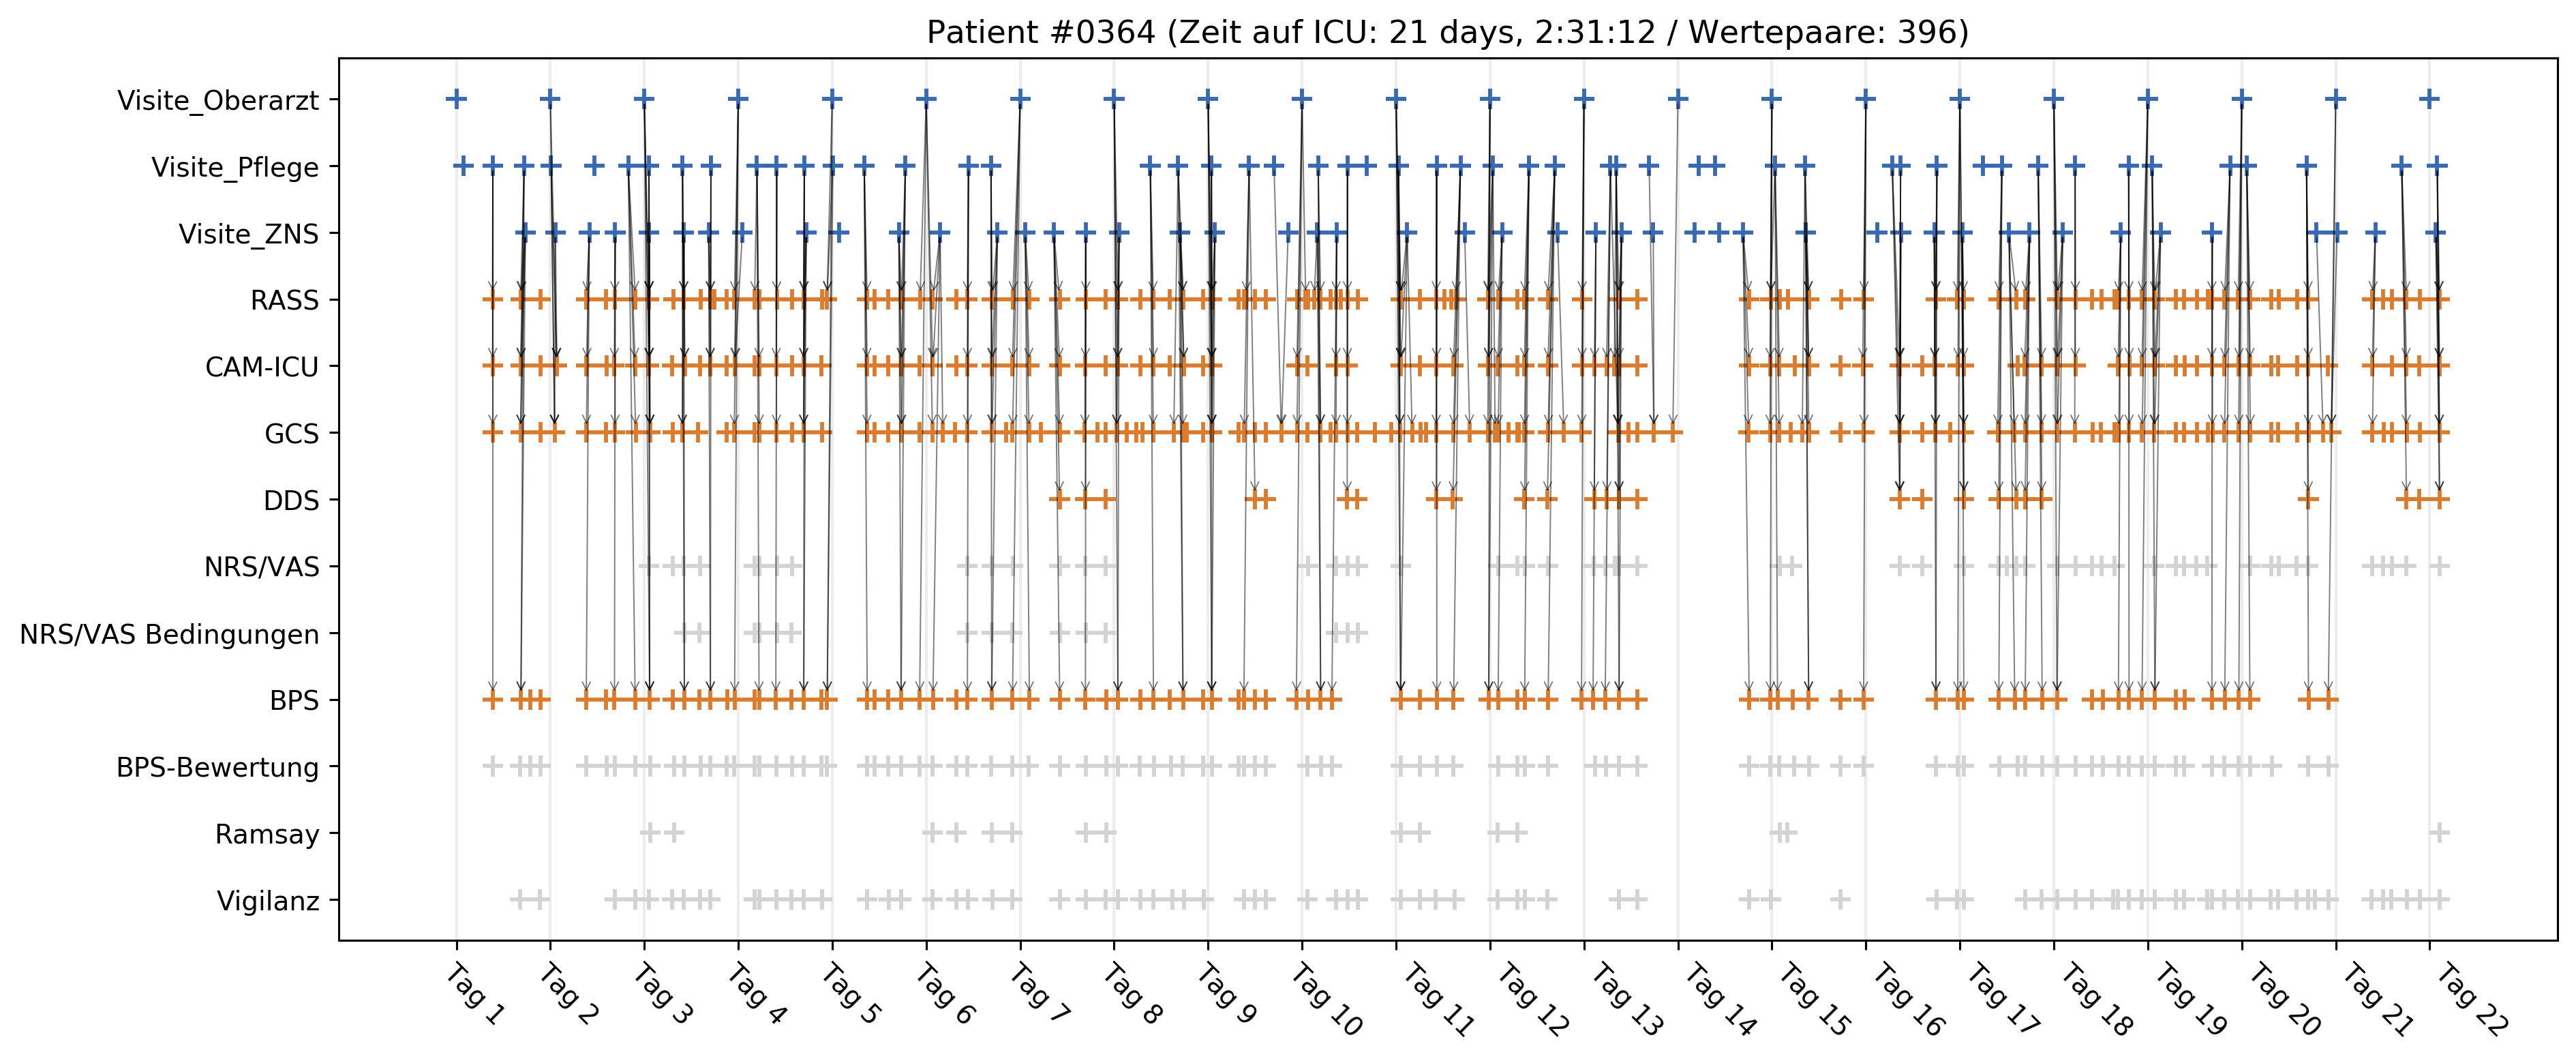
\includegraphics[height=1.87in]{patienten_scatters/patient_0364}} 
    \caption{Übersicht der erfassten Werte einiger Patienten}
    \label{fig:pat_example_scatterplots}
\end{figure}

\section{Genauigkeit der erfassten Daten}\label{section:genauigkeit_der_daten}
Neben einer möglichst genauen, automatischen Vergabe von medizinischen Scores anhand von Visitentexten stellt sich weiterhin die Frage, welche der gegebenen Eingabewerte überhaupt der Wahrheit entsprechen, beziehungsweise diese am genauesten abbilden. Die Modelle, die in Abschnitt \ref{chap-vorgehensweise} beschrieben werden, nehmen die eingetragenen Scores als "absolute Wahrheit"\footnote{Im maschinellen Lernen und in verwandten Bereichen auch als "ground truth" bezeichnet} an. Wir gehen also davon aus, dass diese Eintragungen die Kondition eines Patienten im Zweifelsfall genauer beschreiben als die Visitentexte, die zu einem ähnlichen Zeitpunkt verfasst wurden. Dies stellt allerdings eine Vereinfachung der Situation dar. Im Allgemeinen ist es fast unmöglich, nachträglich zu bestimmen, welcher Wert die Realität widerspiegelt, wenn Score und Text voneinander abweichen. 

Diese Art von Widerspruch tritt in den betrachteten Datensätzen häufig auf und kann mehrere Gründe haben. Zum einen kann es vorkommen, dass Ärzte oder Pflegekräfte aufgrund von Zeitmangel oder Stress einen Text nicht mit der nötigen Gewissenhaftigkeit oder im nötigen Umfang verfassen, um aus den gegebenen Informationen einen Score herzuleiten. Im Extremfall kann es sogar vorkommen, dass Texte oder Scores aus der vorhergehenden Erhebung unverändert übernommen werden, auch wenn sich der Zustand des betreffenden Patienten verändert hat. Wird aber gleichzeitig ein entsprechender Score bzw. Text aktualisiert kommt es zu einem Widerspruch. Ferner ist es selbst ohne menschlichen Fehler möglich, dass Score und Visitentext unterschiedliche Werte indizieren, auch wenn diese zeitlich nah beieinander liegen. Da sich insbesondere auf einer Intensivstation der Zustand eines Patienten sehr schnell ändern kann, kann es durchaus vorkommen, dass sich zwei zeitlich sehr nah beieinanderliegende Eintragungen inhaltlich stark unterscheiden, obwohl beide Werte zum Zeitpunkt ihrer Eintragung als realitätsgetreu angesehen werden können.

Diese Gründe sind nicht weiter Beobachtungsgegenstand der vorliegenden Arbeit. Dennoch muss diese Art von möglichen Unstimmigkeiten in den vorliegenden Daten bei der Konzeption, Entwicklung und Bewertung der Modelle beachtet werden. Insbesondere stellt die Qualität der Eingabedaten, ohne weitere Maßnahmen zur Datenbereinigung, womöglich eine obere Schranke für die Performance der Modelle dar.
	
	
	\chapter{Vorgehensweise}
	Bei der Konzeption eines geeigneten Modells zur Vorhersage medizinischer Scores habe ich mich dafür entschieden, zwei separate, voneinander unabhängige Ansätze zu verfolgen. In Abschnitt \ref{section:baseline} wird die Entwicklung eines einfachen Regressionsmodells auf Basis der sog. Support Vector Machine beschrieben. Abschnitt \ref{section:ELM} beinhaltet die Entwicklung eines Modells basierend auf der Extreme Learning Machine, einem Verfahren, das es ermöglicht, künstliche neuronale Netze mit nur einem hidden layer effizient zu trainieren \citep{huangExtremeLearningMachine2006}. Weiterhin werden in Abschnitt \ref{section:ELM} weitere Methoden zur Vorverarbeitung der Eingabedaten vorgestellt sowie deren Wirkung bewertet. 

\section{Baseline-Modell}\label{section:baseline}
\subsection{Datenaufbereitung}
Die Verarbeitung natürlicher Sprache stellt eine besondere Herausforderung für das maschinelle Lernen dar.
Bevor ein Modell trainiert werden kann muss eine angemessene numerische Repräsentation der Eingabetexte gefunden werden. 

1) vectorization

2) tfidf transformiert jeden eingabetext in einen vector mit gleicher länge. länge=anzahl der unique words.
\subsection{Modell}
scikit learn \citep{JMLR:v12:pedregosa11a}
\subsection{Ergebnisse}
\section{Extreme Learning Machine}\label{section:ELM}

\subsection{Rechtschreibprüfung}
wie viele wörter in den jeweiligen texten, wie viele unique? welches sind die häufigsten? Bla

% bei spell checker eher für einen naiven ansatz entschieden:
% wörter, die öfter als (3) mal vorkommen werden schon als
% richtig angesehen, auch wenn da viele falsch geschriebene
% wörter mit dabei sind. würde man aber nur wörter ansehen
% die noch öfters vorkommen, würde man auch wörter korriegieren
% die eigentlich richtig sind, nur weil sie nicht oft genug
% vorkamen, um als richtig angesehen zu werden:
% 'spannung' > spaltung
% 'verformung' > versorgung
Beschreiben: Verbesserung der featurization der eingabedaten durch word2vec. verbesserung auch durch spell correction, weil es viele falsch geschriebene wörter gibt, die dann in word2vec gar nicht auftauchen. (zeigen, wie sich die anzahl der unbekannten wörter durch spell correction verringert!)

Vergleich unbekannte/bekannte wörter mit spell correction, substitutions etc und ohne.
% * numerische optimierung: Lösungsraum, Bewertungsfunktion
%   * das Gradientenverfahren
%   * stochastic gradient descend
% * Evaluation von ML-Modellen
%       * z.b. cross validation
%       * vermeiden: data leakage

%bla bla bla. "das modell wurde anhand des in Abschnitt 3.2.1 beschriebenen kreuzvalidierungsverfahren getestet."

	
	\chapter{Schluss}
	\dots

\section{Bewertung der Leitlinienadhärenz auf den Intensivstationen der Charité}
\dots

\section{Blick in die Zukunft}
\dots

\chapter{Fazit}
Brilliant formuliert, besonders die Konklusio!


% ## 4) Fazit
%   * Ergebnisse
%   * TODO: Auswertung der Visitentexte: Wo gibt es große Abweichungen von eingetragenem Score/Modell-Vorhersage?
%   * **Anwendung in der Zukunft**
%     * Vorgänge bei Datenerfassung auf ICU optimieren
%     * Erfassung von Qualität der bisher eingetragenen Daten
%     * z.b. einbeziehen der scores in clinicial decision support systems

	\newpage
	\bibliography{literatur}

\end{document}